\documentclass[a4paper, 12pt]{report}
%\usepackage[left=2cm, right=5cm, top=2cm]{geometry}
\usepackage[table, dvipsnames]{xcolor}
\usepackage{soul}
\usepackage{alltt}
\usepackage[utf8]{inputenc}
\usepackage[french]{babel}
\usepackage[pdftex]{graphicx}
\usepackage{fancyhdr}
\usepackage{algorithm}
\usepackage{algorithmic}
\usepackage{cite}
\usepackage{microtype}
\usepackage{makecell}
\usepackage{tikz}
\usepackage{qtree}
\usepackage{newfloat}
\usepackage{moreverb}
\usepackage[T1]{fontenc}
\usepackage{eurosym}

%\usepackage[dvips]{hyperref}

\usepackage{hyperref}
\hypersetup{
colorlinks=true,
linkcolor=red,           
}
\usepackage[outputdir=out]{minted}

\usepackage{pgf-umlsd}
\usetikzlibrary{positioning}
\usetikzlibrary{calc}
%%%%%%%%%%%%%%%%%%%%%%%%%%%%%%%%%%%%%%%%%%%%%%%%%%%%%%%%%%%%%%%%%
%Usage: %%%%%%%%%%%%%%%%%%%%%%%%%%%%%%%%%%%%%%%%%%%%%%%%%%%%%%%%%%%%%%%%%
%Usage: %%%%%%%%%%%%%%%%%%%%%%%%%%%%%%%%%%%%%%%%%%%%%%%%%%%%%%%%%%%%%%%%%
%Usage: \input{../../Function/flow.tex}
%
%	TikZ Functions for pcap2tex  Packets Flow Diagram 
%
%	The Diagramm can be splitted into several pictures in the LaTeX doc.
%	The Picture file (or LaTeX fragment) looks like:
%
%	\begin{tikzpicture}
%	\FLOWPART{./trace/s-h-1}{1}{24}
%	\end{tikzpicture}
%
%	FLOWPART defines:
%		1. Message source file.
%		2. Min and Max Message number for the picture.
%	
%		It is allowed to specify Max > than the full number
%		of the messages in th input file in order to
%		put all data on the one picture.
%
%	All pictures defined by \FLOWPART will share the same 
%	TeX data file.
%
%	The data file should contain the commands: ADDDEV and MESSAGE.
%----------------------------------------------------------------
%
%       \FLOWPART{FileName}{MinMsgNum}{MaxMsgNum}	- 
%			It reinitilizes the counters of devices and messages.
%			It defines the source of data and the range
%			of the displayed messages.
%
%	\ADDDEV{NodeName}	-
%			It adds the device simbol box at the tor row
%			of the picture
%
%	\MESSAGE{\StartNodeNum}{\EndNodeNum}{startTXT}{TXT}{stopTXT}{\StlNum} -
%			It draws the arrow from device StartNodeNum
%			to EndNodeNum.
%			It puts 3 labels on the arrow: {startTXT} @ the begin
%			{TXT} in the middle ; {stopTXT} @ the end of arrow
%----------------------------
%	\ENDLINE	-
%			Used internaly.
%			Compleate the diagram. It draws the vertical lines
%			from the device boxes to the most bottom message.
%			Ë ÐÏÓÌÅÄÎÅÍÕ ÓÏÏÂÝÅÎÉÀ.
%
%================ BEGIN OF FUNCTION DEFINITION ==========================
% 
\pgfdeclarelayer{BGR}
\pgfdeclarelayer{FGR}
\pgfsetlayers{BGR,main,FGR}
%
%
%	ðÒÉÍÅÒ ÉÓÐÏÌØÚÏ×ÁÎÉÑ ÓÌÏ£×:
%	\begin{pgfonlayer}{ layer name }
%	   environment contents
%	\end{pgfonlayer}
%
%
%
\tikzset{
%  5 black boxes on A4 :
        DEV5/.style={rectangle,draw=black!99,fill=blue!9,thin,
                    	inner sep=1pt,
                    	minimum height=5mm, minimum width=30mm,
                    	node distance = 5mm and 5mm, },
% 4 black boxes on A4 :
        DEV4/.style={rectangle,draw=black!99,fill=blue!9,thin,
                        inner sep=1pt,
                        minimum height=5mm, minimum width=30mm,
                        node distance = 17mm and 17mm, },
% 3 black boxes on A4 :
        DEV3/.style={rectangle,draw=black!99,fill=blue!9,thin,
                        inner sep=1pt,
                        minimum height=5mm, minimum width=30mm,
                        node distance = 35mm and 35mm, },
% 2 black boxes on A4 :
        DEV2/.style={rectangle,draw=black!99,fill=blue!9,thin,
                        inner sep=1pt,
                        minimum height=5mm, minimum width=30mm,
                        node distance = 80mm and 80mm, },
%
        NOTE0/.style={font=\normal, text=black, inner sep=0pt,
                node distance = 1mm and 1mm,},
%
% éÍÅÎÁ ÓÔÉÌÅÊ ÄÌÑ ÓÔÒÅÌÙ ÓÏÏÂÝÅÎÉÑ ÄÏÌÖÎÙ ÓÏÈÒÁÎÑÔØÓÑ .
% íÏÖÎÏ ÍÅÎÑÔØ ÔÏÌØËÏ ÎÏÍÅÒ, ËÏÔÏÒÙÊ ÓÌÕÖÉÔ ÁÒÇÕÍÅÎÔÏÍ \MESSAGE .
%
% Blue Message (style 1):
%
        LBL1/.style={font=\scriptsize, text=black, inner sep=0pt,
		node distance = 0.1mm and 0.1mm,},
        TERM1/.style={circle,draw=blue!99,fill=blue!1,thin,
                    	inner sep=1pt, minimum size=1mm, 
			node distance = 0.5mm and 0.5mm, },
        FLOW1/.style={|->,shorten >=2pt,>=stealth,shorten <=2pt,
			thin,draw=blue,fill=blue, },
% Red Message (style 2)
        LBL2/.style={font=\scriptsize, text=black, inner sep=0pt,
			node distance = 0.1mm and 0.1mm,},
        TERM2/.style={draw=red!99,fill=red!1,thin,
                    	inner sep=1pt, minimum size=1.5mm,
			node distance = 0.5mm and 0.5mm, },
        FLOW2/.style={ ->,shorten >=1pt,>=stealth',thin,
                    draw=red!99,fill=red!100 },
% Red Comment (style 3)
        LBL3/.style={font=\scriptsize, text=red!70!black, inner sep=0pt,
			node distance = 0.1mm and 0.1mm,},
        TERM3/.style={starburst,starburst points= 9,starburst point height= 2mm,
			draw=black,fill=yellow!90!red,thin,
                        inner sep=1pt, minimum size=3mm,
                        node distance = 0.1mm and 0.1mm, },
        FLOW3/.style={ - ,shorten >=1pt,>=stealth',thin,
                    draw=black, },
% Black Message (style 0)
        LBL0/.style={font=\scriptsize, text=black, inner sep=0pt,
		node distance = 0.1mm and 0.1mm,},
        TERM0/.style={circle,draw=black!99,fill=black!1,thin,
                    	inner sep=1pt, minimum size=1mm, 
			node distance = 4mm and 0.5mm, },
        FLOW0/.style={ ->,shorten >=1pt,>=stealth',thin,
                    draw=black!99, },
%
% Blue;Dashed;2 Arrows;(style 4):
%
        LBL4/.style={font=\scriptsize, text=black, inner sep=0pt,
                node distance = 0.1mm and 0.1mm,},
        TERM4/.style={circle,draw=blue!99,fill=blue!1,thin,
                        inner sep=1pt, minimum size=1mm,
                        node distance = 0.5mm and 0.5mm, },
        FLOW4/.style={<->,shorten >=2pt,>=stealth,shorten <=2pt,
			densely dashed,semithick,
                        thin,draw=blue,fill=blue, },
% äÌÑ ÒÅÆÅÒÅÎÓÎÙÈ ÌÉÎÉÊ:
% [loosely|densely] dashed|dotted
        BASE/.style={ -,shorten >=1pt,>=stealth',thin,
                     densely dotted },
}
%
%	End of tikzset{/.style}
%
%-----------------------------------------------------------------
% 		÷ÅÒÔÉËÁÌØÎÏÅ ÒÁÓÓÔÏÑÎÉÅ ÍÅÖÄÕ ÓÏÏÂÝÅÎÉÑÍÉ.
\def\VSPACE{5mm}
%
%-----------------------------------------------------------------------------
% Usage : \MESSAGE{\StartNodeNum}{\EndNodeNum}{startTXT}{TXT}{stopTXT}{\StlNum}
%                       1             2                   3               4
%                       1             2           3       4      5        6
%
%
\newcommand{\FLOWPART}[3]{
%
\def\MINMSG{#2}
\def\MAXMSG{#3}
\def\LASTDEV{0}
%
\ifx\theCNTMSG\undefined
  \newcounter{CNTMSG}
\fi
\pgfmathsetcounter{CNTMSG}{0}
%
\ifx\theCNTSHIFT\undefined
  \newcounter{CNTSHIFT}
\fi
%\pgfmathparse{\MINMSG - 1}
\pgfmathsetcounter{CNTSHIFT}{0}
%
\ifx\theCNTDEV\undefined
  \newcounter{CNTDEV}
\fi
\pgfmathsetcounter{CNTDEV}{0}
%
\input{#1}
%
\ENDLINE
}
%------------------------------------------------------
\newcommand{\MESSAGE}[6]{
   \stepcounter{CNTMSG}
   \pgfmathparse{ \MINMSG  < \theCNTMSG + 1 }
   \if 1\pgfmathresult
   \pgfmathparse{ \MAXMSG  > \theCNTMSG - 1 }
   \if 1\pgfmathresult
   \stepcounter{CNTSHIFT}
%
   \pgfmathparse{ #1 > #2 } 
   \if 1\pgfmathresult
	\def\SIDE{right}
	\def\ASIDE{left}
	\def\ANCH{east}
	\def\AANCH{west}
   \else 
	\def\SIDE{left}
	\def\ASIDE{right}
	\def\ANCH{west} 
	\def\AANCH{east}
   \fi
%
   \pgfmathparse{ \theCNTMSG  <  10 }
   \if 1\pgfmathresult
        \def\FNODE{ \theCNTMSG}
   \else
        \def\FNODE{\theCNTMSG}
   \fi
%
   \node (START\theCNTMSG) [TERM#6] at ($ (DEV#1.south) - \theCNTSHIFT *(0,\VSPACE) $) {\tiny \FNODE};
   \node (STOP\theCNTMSG) [TERM#6]   at ($ (DEV#2.south) - \theCNTSHIFT *(0,\VSPACE) $) {\tiny \FNODE};
     \begin{pgfonlayer}{FGR}
     \draw [FLOW#6] (START\theCNTMSG) -- (STOP\theCNTMSG) node (LABEL\theCNTMSG)
             [LBL#6,above,pos=0.5] {#4};
%
%	Start label:
      \node (LABELp\theCNTMSG) [LBL#6,\SIDE =of START\theCNTMSG.\ANCH] {#3};
%	Stop label:
      \node (LABELq\theCNTMSG) [LBL#6,\ASIDE =of STOP\theCNTMSG.\AANCH] {#5};
     \end{pgfonlayer}{FGR}
       \edef\CNTMSGLAST{\theCNTMSG}
  \fi
  \fi
}
%----------------------------------------------------------------------
%	Usage: \ADDDEV{router}
%
\newcommand{\ADDDEV}[2]{
   \stepcounter{CNTDEV}
   \pgfkeyssetvalue{/DEVLIST/\theCNTDEV}{\theCNTDEV}
   \pgfmathparse{\theCNTDEV > 1}
   \if 1\pgfmathresult
        \edef\DEVLIST{\DEVLIST,\theCNTDEV}
	\node (DEV\theCNTDEV) [DEV#2,right=of DEV\LASTDEV] {#1};
   \else
	\edef\DEVLIST{1}
	\node (DEV\theCNTDEV) [DEV#2] {#1};
   \fi
   \edef\LASTDEV{\theCNTDEV};
}
%----------------------------------------------------------------------------
%	ëÏÍÁÎÄÁ ÒÉÓÕÅÔ ÒÅÆÅÒÅÎÓÎÙÅ ÌÉÎÉÉ ×ÎÉÚ ÏÔ ËÁÖÄÏÇÏ ÕÓÔÒÏÊÓÔ×Á. 
%       éÓÐÏÌØÚÏ×ÁÔØ × ËÏÎÃÅ ×ÓÅÈ MESSAGE.
%
\newcommand{\ENDLINE}{
  \begin{pgfonlayer}{BGR}
  \foreach \K in \DEVLIST {
%    \pgfkeysifdefined{/DEVLIST/\K}{
%        \draw [BASE] (DEV\K.south) -- (DEV\K.south |- LABEL\MAXMSG)
	\draw [BASE] (DEV\K.south) -- (DEV\K.south |- START\CNTMSGLAST.south);
% 	}{}
  }
  \end{pgfonlayer}{BGR}
}
%
%================ END OF FUNCTION DEFINITION ==========================
%
%
%	TikZ Functions for pcap2tex  Packets Flow Diagram 
%
%	The Diagramm can be splitted into several pictures in the LaTeX doc.
%	The Picture file (or LaTeX fragment) looks like:
%
%	\begin{tikzpicture}
%	\FLOWPART{./trace/s-h-1}{1}{24}
%	\end{tikzpicture}
%
%	FLOWPART defines:
%		1. Message source file.
%		2. Min and Max Message number for the picture.
%	
%		It is allowed to specify Max > than the full number
%		of the messages in th input file in order to
%		put all data on the one picture.
%
%	All pictures defined by \FLOWPART will share the same 
%	TeX data file.
%
%	The data file should contain the commands: ADDDEV and MESSAGE.
%----------------------------------------------------------------
%
%       \FLOWPART{FileName}{MinMsgNum}{MaxMsgNum}	- 
%			It reinitilizes the counters of devices and messages.
%			It defines the source of data and the range
%			of the displayed messages.
%
%	\ADDDEV{NodeName}	-
%			It adds the device simbol box at the tor row
%			of the picture
%
%	\MESSAGE{\StartNodeNum}{\EndNodeNum}{startTXT}{TXT}{stopTXT}{\StlNum} -
%			It draws the arrow from device StartNodeNum
%			to EndNodeNum.
%			It puts 3 labels on the arrow: {startTXT} @ the begin
%			{TXT} in the middle ; {stopTXT} @ the end of arrow
%----------------------------
%	\ENDLINE	-
%			Used internaly.
%			Compleate the diagram. It draws the vertical lines
%			from the device boxes to the most bottom message.
%			Ë ÐÏÓÌÅÄÎÅÍÕ ÓÏÏÂÝÅÎÉÀ.
%
%================ BEGIN OF FUNCTION DEFINITION ==========================
% 
\pgfdeclarelayer{BGR}
\pgfdeclarelayer{FGR}
\pgfsetlayers{BGR,main,FGR}
%
%
%	ðÒÉÍÅÒ ÉÓÐÏÌØÚÏ×ÁÎÉÑ ÓÌÏ£×:
%	\begin{pgfonlayer}{ layer name }
%	   environment contents
%	\end{pgfonlayer}
%
%
%
\tikzset{
%  5 black boxes on A4 :
        DEV5/.style={rectangle,draw=black!99,fill=blue!9,thin,
                    	inner sep=1pt,
                    	minimum height=5mm, minimum width=30mm,
                    	node distance = 5mm and 5mm, },
% 4 black boxes on A4 :
        DEV4/.style={rectangle,draw=black!99,fill=blue!9,thin,
                        inner sep=1pt,
                        minimum height=5mm, minimum width=30mm,
                        node distance = 17mm and 17mm, },
% 3 black boxes on A4 :
        DEV3/.style={rectangle,draw=black!99,fill=blue!9,thin,
                        inner sep=1pt,
                        minimum height=5mm, minimum width=30mm,
                        node distance = 35mm and 35mm, },
% 2 black boxes on A4 :
        DEV2/.style={rectangle,draw=black!99,fill=blue!9,thin,
                        inner sep=1pt,
                        minimum height=5mm, minimum width=30mm,
                        node distance = 80mm and 80mm, },
%
        NOTE0/.style={font=\normal, text=black, inner sep=0pt,
                node distance = 1mm and 1mm,},
%
% éÍÅÎÁ ÓÔÉÌÅÊ ÄÌÑ ÓÔÒÅÌÙ ÓÏÏÂÝÅÎÉÑ ÄÏÌÖÎÙ ÓÏÈÒÁÎÑÔØÓÑ .
% íÏÖÎÏ ÍÅÎÑÔØ ÔÏÌØËÏ ÎÏÍÅÒ, ËÏÔÏÒÙÊ ÓÌÕÖÉÔ ÁÒÇÕÍÅÎÔÏÍ \MESSAGE .
%
% Blue Message (style 1):
%
        LBL1/.style={font=\scriptsize, text=black, inner sep=0pt,
		node distance = 0.1mm and 0.1mm,},
        TERM1/.style={circle,draw=blue!99,fill=blue!1,thin,
                    	inner sep=1pt, minimum size=1mm, 
			node distance = 0.5mm and 0.5mm, },
        FLOW1/.style={|->,shorten >=2pt,>=stealth,shorten <=2pt,
			thin,draw=blue,fill=blue, },
% Red Message (style 2)
        LBL2/.style={font=\scriptsize, text=black, inner sep=0pt,
			node distance = 0.1mm and 0.1mm,},
        TERM2/.style={draw=red!99,fill=red!1,thin,
                    	inner sep=1pt, minimum size=1.5mm,
			node distance = 0.5mm and 0.5mm, },
        FLOW2/.style={ ->,shorten >=1pt,>=stealth',thin,
                    draw=red!99,fill=red!100 },
% Red Comment (style 3)
        LBL3/.style={font=\scriptsize, text=red!70!black, inner sep=0pt,
			node distance = 0.1mm and 0.1mm,},
        TERM3/.style={starburst,starburst points= 9,starburst point height= 2mm,
			draw=black,fill=yellow!90!red,thin,
                        inner sep=1pt, minimum size=3mm,
                        node distance = 0.1mm and 0.1mm, },
        FLOW3/.style={ - ,shorten >=1pt,>=stealth',thin,
                    draw=black, },
% Black Message (style 0)
        LBL0/.style={font=\scriptsize, text=black, inner sep=0pt,
		node distance = 0.1mm and 0.1mm,},
        TERM0/.style={circle,draw=black!99,fill=black!1,thin,
                    	inner sep=1pt, minimum size=1mm, 
			node distance = 4mm and 0.5mm, },
        FLOW0/.style={ ->,shorten >=1pt,>=stealth',thin,
                    draw=black!99, },
%
% Blue;Dashed;2 Arrows;(style 4):
%
        LBL4/.style={font=\scriptsize, text=black, inner sep=0pt,
                node distance = 0.1mm and 0.1mm,},
        TERM4/.style={circle,draw=blue!99,fill=blue!1,thin,
                        inner sep=1pt, minimum size=1mm,
                        node distance = 0.5mm and 0.5mm, },
        FLOW4/.style={<->,shorten >=2pt,>=stealth,shorten <=2pt,
			densely dashed,semithick,
                        thin,draw=blue,fill=blue, },
% äÌÑ ÒÅÆÅÒÅÎÓÎÙÈ ÌÉÎÉÊ:
% [loosely|densely] dashed|dotted
        BASE/.style={ -,shorten >=1pt,>=stealth',thin,
                     densely dotted },
}
%
%	End of tikzset{/.style}
%
%-----------------------------------------------------------------
% 		÷ÅÒÔÉËÁÌØÎÏÅ ÒÁÓÓÔÏÑÎÉÅ ÍÅÖÄÕ ÓÏÏÂÝÅÎÉÑÍÉ.
\def\VSPACE{5mm}
%
%-----------------------------------------------------------------------------
% Usage : \MESSAGE{\StartNodeNum}{\EndNodeNum}{startTXT}{TXT}{stopTXT}{\StlNum}
%                       1             2                   3               4
%                       1             2           3       4      5        6
%
%
\newcommand{\FLOWPART}[3]{
%
\def\MINMSG{#2}
\def\MAXMSG{#3}
\def\LASTDEV{0}
%
\ifx\theCNTMSG\undefined
  \newcounter{CNTMSG}
\fi
\pgfmathsetcounter{CNTMSG}{0}
%
\ifx\theCNTSHIFT\undefined
  \newcounter{CNTSHIFT}
\fi
%\pgfmathparse{\MINMSG - 1}
\pgfmathsetcounter{CNTSHIFT}{0}
%
\ifx\theCNTDEV\undefined
  \newcounter{CNTDEV}
\fi
\pgfmathsetcounter{CNTDEV}{0}
%
\input{#1}
%
\ENDLINE
}
%------------------------------------------------------
\newcommand{\MESSAGE}[6]{
   \stepcounter{CNTMSG}
   \pgfmathparse{ \MINMSG  < \theCNTMSG + 1 }
   \if 1\pgfmathresult
   \pgfmathparse{ \MAXMSG  > \theCNTMSG - 1 }
   \if 1\pgfmathresult
   \stepcounter{CNTSHIFT}
%
   \pgfmathparse{ #1 > #2 } 
   \if 1\pgfmathresult
	\def\SIDE{right}
	\def\ASIDE{left}
	\def\ANCH{east}
	\def\AANCH{west}
   \else 
	\def\SIDE{left}
	\def\ASIDE{right}
	\def\ANCH{west} 
	\def\AANCH{east}
   \fi
%
   \pgfmathparse{ \theCNTMSG  <  10 }
   \if 1\pgfmathresult
        \def\FNODE{ \theCNTMSG}
   \else
        \def\FNODE{\theCNTMSG}
   \fi
%
   \node (START\theCNTMSG) [TERM#6] at ($ (DEV#1.south) - \theCNTSHIFT *(0,\VSPACE) $) {\tiny \FNODE};
   \node (STOP\theCNTMSG) [TERM#6]   at ($ (DEV#2.south) - \theCNTSHIFT *(0,\VSPACE) $) {\tiny \FNODE};
     \begin{pgfonlayer}{FGR}
     \draw [FLOW#6] (START\theCNTMSG) -- (STOP\theCNTMSG) node (LABEL\theCNTMSG)
             [LBL#6,above,pos=0.5] {#4};
%
%	Start label:
      \node (LABELp\theCNTMSG) [LBL#6,\SIDE =of START\theCNTMSG.\ANCH] {#3};
%	Stop label:
      \node (LABELq\theCNTMSG) [LBL#6,\ASIDE =of STOP\theCNTMSG.\AANCH] {#5};
     \end{pgfonlayer}{FGR}
       \edef\CNTMSGLAST{\theCNTMSG}
  \fi
  \fi
}
%----------------------------------------------------------------------
%	Usage: \ADDDEV{router}
%
\newcommand{\ADDDEV}[2]{
   \stepcounter{CNTDEV}
   \pgfkeyssetvalue{/DEVLIST/\theCNTDEV}{\theCNTDEV}
   \pgfmathparse{\theCNTDEV > 1}
   \if 1\pgfmathresult
        \edef\DEVLIST{\DEVLIST,\theCNTDEV}
	\node (DEV\theCNTDEV) [DEV#2,right=of DEV\LASTDEV] {#1};
   \else
	\edef\DEVLIST{1}
	\node (DEV\theCNTDEV) [DEV#2] {#1};
   \fi
   \edef\LASTDEV{\theCNTDEV};
}
%----------------------------------------------------------------------------
%	ëÏÍÁÎÄÁ ÒÉÓÕÅÔ ÒÅÆÅÒÅÎÓÎÙÅ ÌÉÎÉÉ ×ÎÉÚ ÏÔ ËÁÖÄÏÇÏ ÕÓÔÒÏÊÓÔ×Á. 
%       éÓÐÏÌØÚÏ×ÁÔØ × ËÏÎÃÅ ×ÓÅÈ MESSAGE.
%
\newcommand{\ENDLINE}{
  \begin{pgfonlayer}{BGR}
  \foreach \K in \DEVLIST {
%    \pgfkeysifdefined{/DEVLIST/\K}{
%        \draw [BASE] (DEV\K.south) -- (DEV\K.south |- LABEL\MAXMSG)
	\draw [BASE] (DEV\K.south) -- (DEV\K.south |- START\CNTMSGLAST.south);
% 	}{}
  }
  \end{pgfonlayer}{BGR}
}
%
%================ END OF FUNCTION DEFINITION ==========================
%
%
%	TikZ Functions for pcap2tex  Packets Flow Diagram 
%
%	The Diagramm can be splitted into several pictures in the LaTeX doc.
%	The Picture file (or LaTeX fragment) looks like:
%
%	\begin{tikzpicture}
%	\FLOWPART{./trace/s-h-1}{1}{24}
%	\end{tikzpicture}
%
%	FLOWPART defines:
%		1. Message source file.
%		2. Min and Max Message number for the picture.
%	
%		It is allowed to specify Max > than the full number
%		of the messages in th input file in order to
%		put all data on the one picture.
%
%	All pictures defined by \FLOWPART will share the same 
%	TeX data file.
%
%	The data file should contain the commands: ADDDEV and MESSAGE.
%----------------------------------------------------------------
%
%       \FLOWPART{FileName}{MinMsgNum}{MaxMsgNum}	- 
%			It reinitilizes the counters of devices and messages.
%			It defines the source of data and the range
%			of the displayed messages.
%
%	\ADDDEV{NodeName}	-
%			It adds the device simbol box at the tor row
%			of the picture
%
%	\MESSAGE{\StartNodeNum}{\EndNodeNum}{startTXT}{TXT}{stopTXT}{\StlNum} -
%			It draws the arrow from device StartNodeNum
%			to EndNodeNum.
%			It puts 3 labels on the arrow: {startTXT} @ the begin
%			{TXT} in the middle ; {stopTXT} @ the end of arrow
%----------------------------
%	\ENDLINE	-
%			Used internaly.
%			Compleate the diagram. It draws the vertical lines
%			from the device boxes to the most bottom message.
%			Ë ÐÏÓÌÅÄÎÅÍÕ ÓÏÏÂÝÅÎÉÀ.
%
%================ BEGIN OF FUNCTION DEFINITION ==========================
% 
\pgfdeclarelayer{BGR}
\pgfdeclarelayer{FGR}
\pgfsetlayers{BGR,main,FGR}
%
%
%	ðÒÉÍÅÒ ÉÓÐÏÌØÚÏ×ÁÎÉÑ ÓÌÏ£×:
%	\begin{pgfonlayer}{ layer name }
%	   environment contents
%	\end{pgfonlayer}
%
%
%
\tikzset{
%  5 black boxes on A4 :
        DEV5/.style={rectangle,draw=black!99,fill=blue!9,thin,
                    	inner sep=1pt,
                    	minimum height=5mm, minimum width=30mm,
                    	node distance = 5mm and 5mm, },
% 4 black boxes on A4 :
        DEV4/.style={rectangle,draw=black!99,fill=blue!9,thin,
                        inner sep=1pt,
                        minimum height=5mm, minimum width=30mm,
                        node distance = 17mm and 17mm, },
% 3 black boxes on A4 :
        DEV3/.style={rectangle,draw=black!99,fill=blue!9,thin,
                        inner sep=1pt,
                        minimum height=5mm, minimum width=30mm,
                        node distance = 35mm and 35mm, },
% 2 black boxes on A4 :
        DEV2/.style={rectangle,draw=black!99,fill=blue!9,thin,
                        inner sep=1pt,
                        minimum height=5mm, minimum width=30mm,
                        node distance = 80mm and 80mm, },
%
        NOTE0/.style={font=\normal, text=black, inner sep=0pt,
                node distance = 1mm and 1mm,},
%
% éÍÅÎÁ ÓÔÉÌÅÊ ÄÌÑ ÓÔÒÅÌÙ ÓÏÏÂÝÅÎÉÑ ÄÏÌÖÎÙ ÓÏÈÒÁÎÑÔØÓÑ .
% íÏÖÎÏ ÍÅÎÑÔØ ÔÏÌØËÏ ÎÏÍÅÒ, ËÏÔÏÒÙÊ ÓÌÕÖÉÔ ÁÒÇÕÍÅÎÔÏÍ \MESSAGE .
%
% Blue Message (style 1):
%
        LBL1/.style={font=\scriptsize, text=black, inner sep=0pt,
		node distance = 0.1mm and 0.1mm,},
        TERM1/.style={circle,draw=blue!99,fill=blue!1,thin,
                    	inner sep=1pt, minimum size=1mm, 
			node distance = 0.5mm and 0.5mm, },
        FLOW1/.style={|->,shorten >=2pt,>=stealth,shorten <=2pt,
			thin,draw=blue,fill=blue, },
% Red Message (style 2)
        LBL2/.style={font=\scriptsize, text=black, inner sep=0pt,
			node distance = 0.1mm and 0.1mm,},
        TERM2/.style={draw=red!99,fill=red!1,thin,
                    	inner sep=1pt, minimum size=1.5mm,
			node distance = 0.5mm and 0.5mm, },
        FLOW2/.style={ ->,shorten >=1pt,>=stealth',thin,
                    draw=red!99,fill=red!100 },
% Red Comment (style 3)
        LBL3/.style={font=\scriptsize, text=red!70!black, inner sep=0pt,
			node distance = 0.1mm and 0.1mm,},
        TERM3/.style={starburst,starburst points= 9,starburst point height= 2mm,
			draw=black,fill=yellow!90!red,thin,
                        inner sep=1pt, minimum size=3mm,
                        node distance = 0.1mm and 0.1mm, },
        FLOW3/.style={ - ,shorten >=1pt,>=stealth',thin,
                    draw=black, },
% Black Message (style 0)
        LBL0/.style={font=\scriptsize, text=black, inner sep=0pt,
		node distance = 0.1mm and 0.1mm,},
        TERM0/.style={circle,draw=black!99,fill=black!1,thin,
                    	inner sep=1pt, minimum size=1mm, 
			node distance = 4mm and 0.5mm, },
        FLOW0/.style={ ->,shorten >=1pt,>=stealth',thin,
                    draw=black!99, },
%
% Blue;Dashed;2 Arrows;(style 4):
%
        LBL4/.style={font=\scriptsize, text=black, inner sep=0pt,
                node distance = 0.1mm and 0.1mm,},
        TERM4/.style={circle,draw=blue!99,fill=blue!1,thin,
                        inner sep=1pt, minimum size=1mm,
                        node distance = 0.5mm and 0.5mm, },
        FLOW4/.style={<->,shorten >=2pt,>=stealth,shorten <=2pt,
			densely dashed,semithick,
                        thin,draw=blue,fill=blue, },
% äÌÑ ÒÅÆÅÒÅÎÓÎÙÈ ÌÉÎÉÊ:
% [loosely|densely] dashed|dotted
        BASE/.style={ -,shorten >=1pt,>=stealth',thin,
                     densely dotted },
}
%
%	End of tikzset{/.style}
%
%-----------------------------------------------------------------
% 		÷ÅÒÔÉËÁÌØÎÏÅ ÒÁÓÓÔÏÑÎÉÅ ÍÅÖÄÕ ÓÏÏÂÝÅÎÉÑÍÉ.
\def\VSPACE{5mm}
%
%-----------------------------------------------------------------------------
% Usage : \MESSAGE{\StartNodeNum}{\EndNodeNum}{startTXT}{TXT}{stopTXT}{\StlNum}
%                       1             2                   3               4
%                       1             2           3       4      5        6
%
%
\newcommand{\FLOWPART}[3]{
%
\def\MINMSG{#2}
\def\MAXMSG{#3}
\def\LASTDEV{0}
%
\ifx\theCNTMSG\undefined
  \newcounter{CNTMSG}
\fi
\pgfmathsetcounter{CNTMSG}{0}
%
\ifx\theCNTSHIFT\undefined
  \newcounter{CNTSHIFT}
\fi
%\pgfmathparse{\MINMSG - 1}
\pgfmathsetcounter{CNTSHIFT}{0}
%
\ifx\theCNTDEV\undefined
  \newcounter{CNTDEV}
\fi
\pgfmathsetcounter{CNTDEV}{0}
%
\input{#1}
%
\ENDLINE
}
%------------------------------------------------------
\newcommand{\MESSAGE}[6]{
   \stepcounter{CNTMSG}
   \pgfmathparse{ \MINMSG  < \theCNTMSG + 1 }
   \if 1\pgfmathresult
   \pgfmathparse{ \MAXMSG  > \theCNTMSG - 1 }
   \if 1\pgfmathresult
   \stepcounter{CNTSHIFT}
%
   \pgfmathparse{ #1 > #2 } 
   \if 1\pgfmathresult
	\def\SIDE{right}
	\def\ASIDE{left}
	\def\ANCH{east}
	\def\AANCH{west}
   \else 
	\def\SIDE{left}
	\def\ASIDE{right}
	\def\ANCH{west} 
	\def\AANCH{east}
   \fi
%
   \pgfmathparse{ \theCNTMSG  <  10 }
   \if 1\pgfmathresult
        \def\FNODE{ \theCNTMSG}
   \else
        \def\FNODE{\theCNTMSG}
   \fi
%
   \node (START\theCNTMSG) [TERM#6] at ($ (DEV#1.south) - \theCNTSHIFT *(0,\VSPACE) $) {\tiny \FNODE};
   \node (STOP\theCNTMSG) [TERM#6]   at ($ (DEV#2.south) - \theCNTSHIFT *(0,\VSPACE) $) {\tiny \FNODE};
     \begin{pgfonlayer}{FGR}
     \draw [FLOW#6] (START\theCNTMSG) -- (STOP\theCNTMSG) node (LABEL\theCNTMSG)
             [LBL#6,above,pos=0.5] {#4};
%
%	Start label:
      \node (LABELp\theCNTMSG) [LBL#6,\SIDE =of START\theCNTMSG.\ANCH] {#3};
%	Stop label:
      \node (LABELq\theCNTMSG) [LBL#6,\ASIDE =of STOP\theCNTMSG.\AANCH] {#5};
     \end{pgfonlayer}{FGR}
       \edef\CNTMSGLAST{\theCNTMSG}
  \fi
  \fi
}
%----------------------------------------------------------------------
%	Usage: \ADDDEV{router}
%
\newcommand{\ADDDEV}[2]{
   \stepcounter{CNTDEV}
   \pgfkeyssetvalue{/DEVLIST/\theCNTDEV}{\theCNTDEV}
   \pgfmathparse{\theCNTDEV > 1}
   \if 1\pgfmathresult
        \edef\DEVLIST{\DEVLIST,\theCNTDEV}
	\node (DEV\theCNTDEV) [DEV#2,right=of DEV\LASTDEV] {#1};
   \else
	\edef\DEVLIST{1}
	\node (DEV\theCNTDEV) [DEV#2] {#1};
   \fi
   \edef\LASTDEV{\theCNTDEV};
}
%----------------------------------------------------------------------------
%	ëÏÍÁÎÄÁ ÒÉÓÕÅÔ ÒÅÆÅÒÅÎÓÎÙÅ ÌÉÎÉÉ ×ÎÉÚ ÏÔ ËÁÖÄÏÇÏ ÕÓÔÒÏÊÓÔ×Á. 
%       éÓÐÏÌØÚÏ×ÁÔØ × ËÏÎÃÅ ×ÓÅÈ MESSAGE.
%
\newcommand{\ENDLINE}{
  \begin{pgfonlayer}{BGR}
  \foreach \K in \DEVLIST {
%    \pgfkeysifdefined{/DEVLIST/\K}{
%        \draw [BASE] (DEV\K.south) -- (DEV\K.south |- LABEL\MAXMSG)
	\draw [BASE] (DEV\K.south) -- (DEV\K.south |- START\CNTMSGLAST.south);
% 	}{}
  }
  \end{pgfonlayer}{BGR}
}
%
%================ END OF FUNCTION DEFINITION ==========================
%


%\setcounter{tocdepth}{5} %pour l'apparition dans la table des matières des susubsections
%\setcounter{secnumdepth}{5}%pour la numérotation dans le corps du document des susubsections

\definecolor{myGray}{RGB}{229, 229, 229}

\newcommand{\esp}{\textsc{esp32}}
\newcommand{\espmesh}{\textsc{esp-mesh}}
\newcommand{\mac}{\textsc{mac}}
\newcommand{\rssi}{\textsc{rssi}}
\newcommand{\mesh}{\textsc{mesh}}
\newcommand{\espnow}{\textsc{esp-now}}
\newcommand{\wifi}{Wi-Fi}
\newcommand{\aodv}{\textsc{aodv}}
\newcommand{\todo}[1]{\textcolor{ForestGreen}{\textbf{TODO: #1}}}
\newcommand{\rreq}{\textsc{rreq}}
\newcommand{\rrep}{\textsc{rrep}}
\newcommand{\rerr}{\textsc{rerr}}
\newcommand{\ip}{\textsc{ip}}



\DeclareFloatingEnvironment[fileext=lod]{diagram}

\begin{document}

\begin{titlepage}
\begin{center}

{\Large Université de Mons}\\[1ex]
{\Large Faculté des sciences}\\[1ex]
{\Large Département d'Informatique}\\[1ex]
{\Large Service de réseaux et télécommunications}\\[2.5cm]

\newcommand{\HRule}{\rule{\linewidth}{0.3mm}}
% Title
\HRule \\[0.3cm]
{ \LARGE \bfseries Réseau Wi-Fi multi-sauts sur plateforme ESP \\[0.3cm]}
\HRule \\[1.5cm]

% Author and supervisor
\begin{minipage}[t]{0.45\textwidth}
\begin{flushleft} \large
\emph{Directeur:}\\
Bruno \textsc{Quoitin}\\
\vspace{1.2cm}
\emph{Rapporteurs:}\\
Alain \textsc{Buyse}\\
Jeremy \textsc{Dubrulle}\\
\end{flushleft}
\end{minipage}
\begin{minipage}[t]{0.45\textwidth}
\begin{flushright} \large
\emph{Auteur:} \\
Arnaud \textsc{Palgen}
\end{flushright}
\end{minipage}\\[2ex]

\vfill

% Bottom of the page
\begin{center}
\begin{tabular}[t]{c c c}

\includegraphics[height=1.5cm]{images/logoumons.jpg} &
\hspace{0.3cm} &

\includegraphics[height=1.5cm]{images/logofs.jpg}
\end{tabular}
\end{center}~\\
 
{\large Année académique 2019-2020}

\end{center}
\end{titlepage}

\chapter*{Introduction}
    Un réseau \wifi\ traditionnel (voir Fig. \ref{traditional-network-pic}) est composé
    d'un noeud central, le point d'accès (AP) qui est
    directement connecté à tous les autres noeuds (stations) du réseau.
    L'AP a alors pour rôle d'acheminer les paquets d'une station à une autre
    mais aussi des paquets vers des adresses \textsc{ip} externe au réseau.
    Un inconvénient de ces réseaux est qu'ils ont une couverture limitée car chaque station
    doit se trouver à portée de l'AP.\\

    \begin{figure}[H]
        \centering
        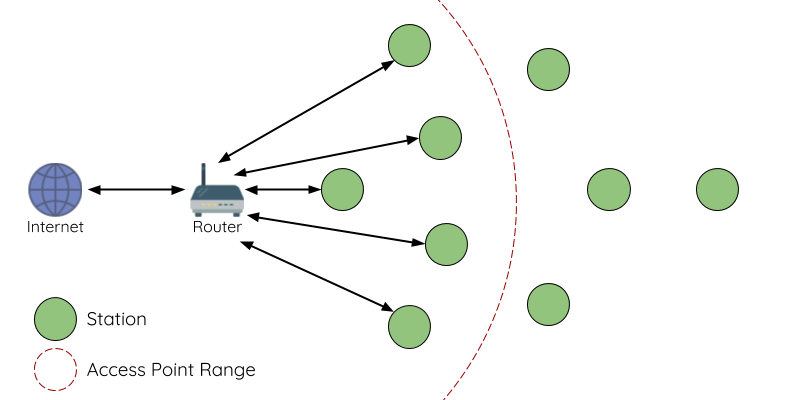
\includegraphics[scale=0.4]{images/traditional-network-architecture.png}
        \caption{Réseau \wifi\ traditionnel \cite{esp-mesh}}
        \label{traditional-network-pic}
    \end{figure}

    L'objectif de ce projet est de concevoir un réseau \mesh\ multi-sauts (voir Fig. \ref{mesh-network-pic})
    \footnote{Notez que sur la figure, un seul noeud fait office d'interface
    entre le réseau \mesh\ et le réseaux \textsc{ip} externe. Ce n'est cependant pas toujours
    le cas} qui n'a pas ce problème. 
    Un réseau \mesh\ multi-sauts est un réseau où tous les noeuds peuvent communiquer avec tous les
    autres noeuds à la portée de leur radio. Chaque noeud peut ainsi acheminer
    les paquets de données de ses voisins vers le noeud suivant et ainsi de suite, jusqu'à ce qu'ils
    atteigent leurs destinations. Les routes utilisées pour acheminer les paquets sont obtenus à l'aide
    d'un protocole de routage.\\

    \begin{figure}[H]
        \centering
        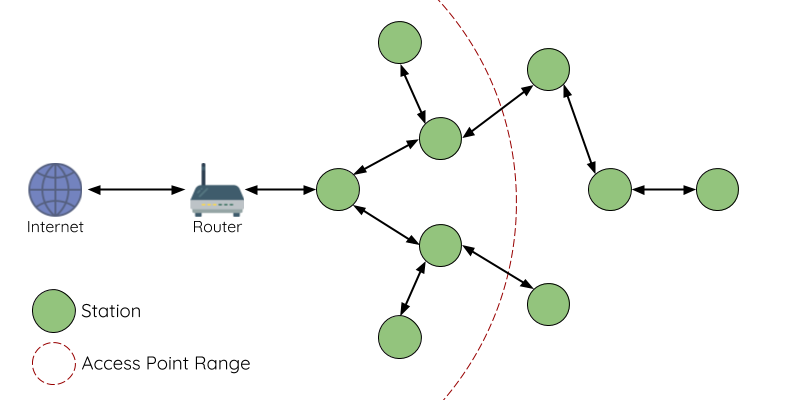
\includegraphics[scale=0.4]{images/mesh-esp-mesh-network-architecture.png}
        \caption{Réseau \mesh\ \cite{esp-mesh}}
        \label{mesh-network-pic}
    \end{figure}

    
    Pour ce projet, les noeuds du réseau \mesh\ seront des microcontrôleurs \wifi. 
    L'\esp\ d'Espressif sera utilisé en raison de son très faible coût et
    ses outils pemettant d'obtenir une consommation électrique ultra-faible.\\

    Dans un premier temps, nous devrons choisir un protocole adapté à ce type
    de réseau et à l'\esp. En effet, il existe une multitude de protocoles
    \mesh\ dans la littérature scientifique.\\

    Une fois choisi, nous implémenterons ce protocole pour créer un
    réseau fonctionnel. Le réseau ainsi créé sera testé pour en évaluer sa performance et ses fonctionnalités.\\

    Enfin, nous nous attarderons sur l'économie d'énergie du microcontrôleur pour
    que notre réseau puisse être alimenté par batterie.


\tableofcontents
\newpage

\chapter{Etat de l'Art}

%%%%%%%%%%%%%%%%%%%%%%%%%%%%%%%%%%%%%%%%%%%%%%%%%%%%%%%%%%%%%%%%%%%%%%%%%%%%%%%
\section{Présentation de l'ESP}
    \textbf{Aperçu}

    \begin{figure}[H]
        \centering
        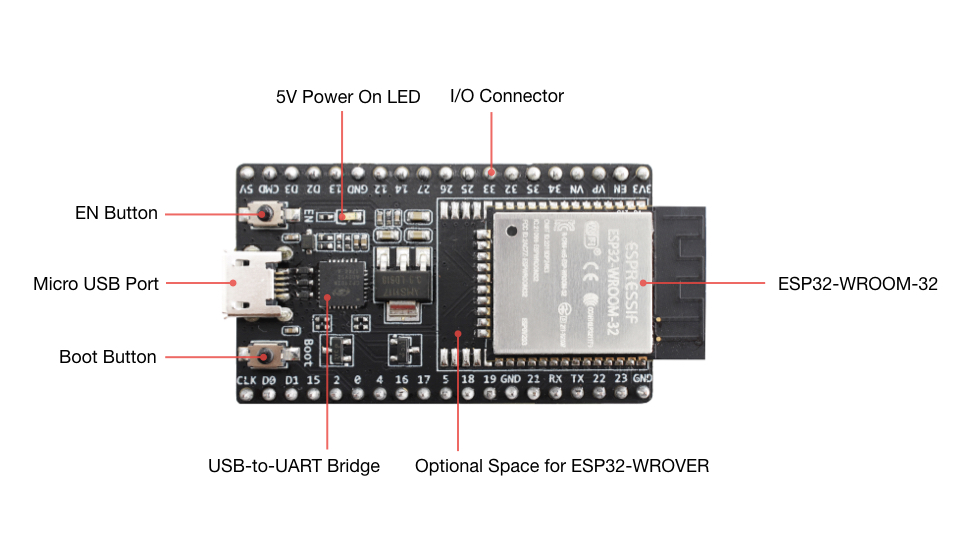
\includegraphics[scale=0.3]{images/esp32-devkitc.jpg}
        \caption{ESP32-DevKitC V4 with ESP32-WROOM-32 module
            \cite{esp32-gettingStarted_w}}
        \label{esp32_img}
    \end{figure}
    Comme dit plus haut, les noeuds de notre réseau seront des \esp.
    Pour ce projet, nous utilisons un kit de développement (Fig. \ref{esp32_img}) équipé d'un
    \esp\textsc{-wroom32}, développé par Espressif. L'\esp\textsc{-wroom32}
    un System-on-Chip (SoC), c'est à dire un circuit intégré rassemblant plusieurs
    composants comme des entrées/sorties, de la mémoire \textsc{ram}, micorprocesseurs,
    microcontrôleurs, etc.
    %todo prix
    Il a été choisis pour son faible coût et sa conception adaptée à l'Internet des Objets (IoT). 
    En effet, en plus de supporter le \wifi\ et le Bluetooth 2.4GHz,
    sa consommation en énergie est faible et il possède des mécanismes permettant de l'économiser. %et il possède plusieurs modes de fonctionnement.
    %permettant de la réduire (voir Table \ref{Consumption_PowerModes}).
    La table \ref{spec} fournit ses spécifications.
    \begin{table}[H]
        \centering
        \begin{tabular}{|c|c|}
            \hline
            \rowcolor{lightgray}
            Element & Spécification\\ \hline
            WiFi & 802.11 b/g/n (802.11n jusqu'à 150 Mbps)\\ \hline
            Bluetooth & Bluetooth v4.2 BR/EDR and BLE specification\\ \hline
            CPU & 2 micorprocesseurs Xtensa \up{\tiny{\textregistered}} 32-bit LX6\\ \hline
            Interfaces & \makecell{SD card, UART, SPI, SDIO, I2C, LED PWM, Motor PWM, I2S,IR, \\
                pulse counter, GPIO, capacitive touch sensor, ADC, DAC}\\ \hline
            \makecell{Tension de \\fonctionnement} & $3.0V \sim 3.6V$\\ \hline
        \end{tabular}
        \caption{Spécification de l'\esp\textsc{-wroom32} \cite{esp32WROOM_datasheet}}
        \label{spec}
    \end{table}
    \textbf{Schéma-bloc}
    \begin{figure}[H]
        \centering
        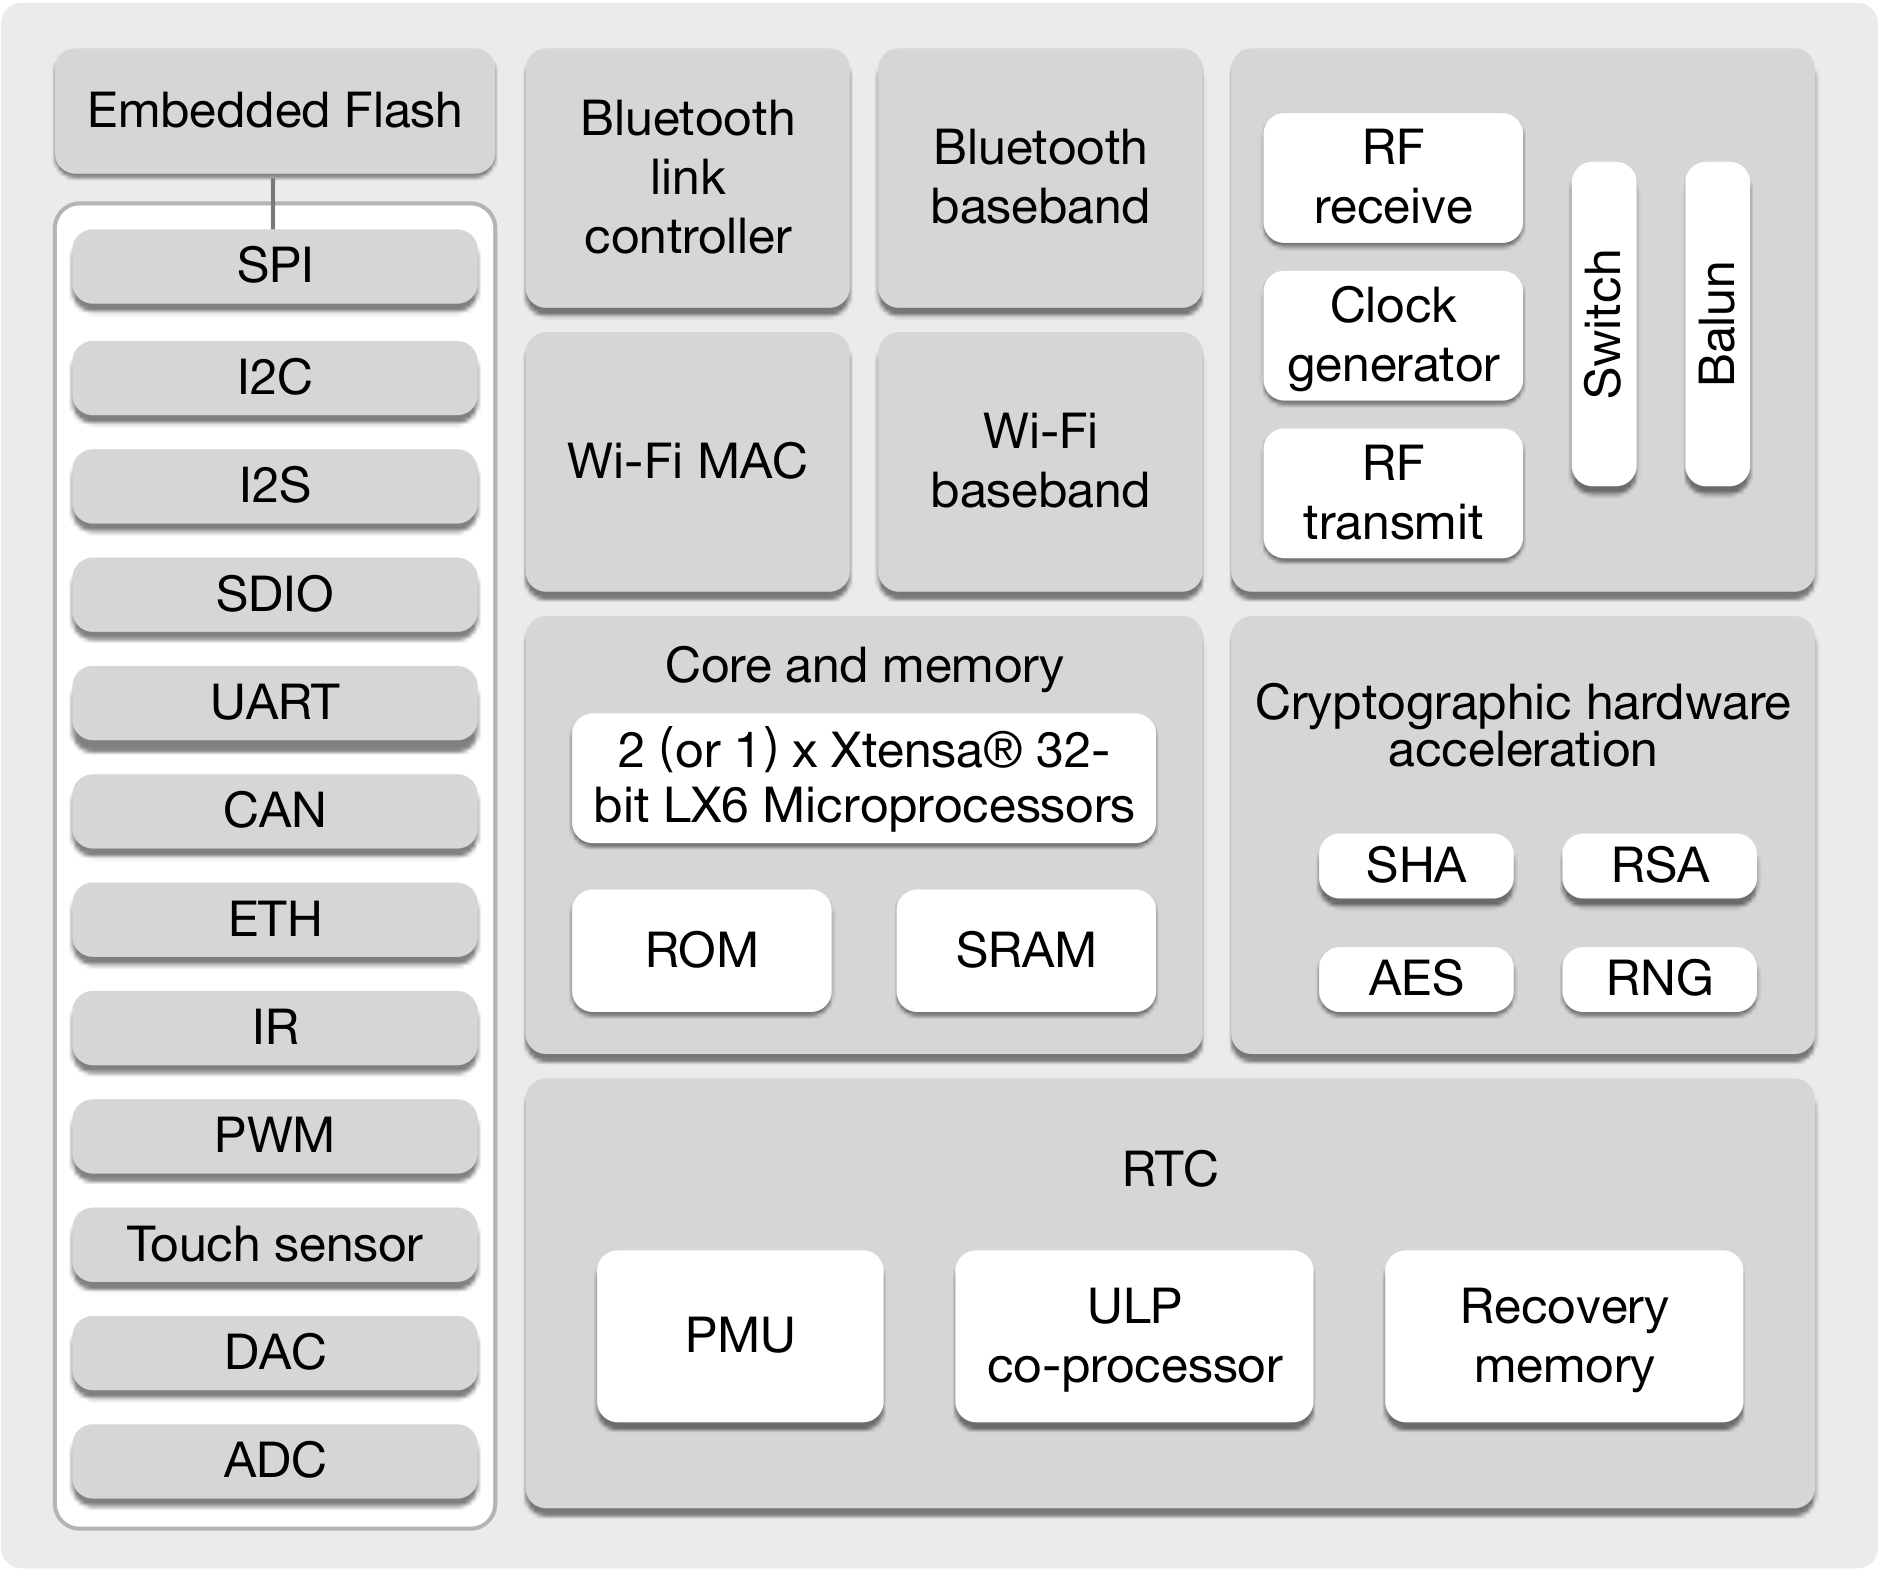
\includegraphics[scale=0.15]{images/esp32-blockDiagram.png}
        \caption{Schéma-bloc \cite{esp32_datasheet}}
        %\label{}
    \end{figure}

    \textbf{Mémoire}\cite{esp32WROOM_datasheet}\\
        La mémoire interne inclut:
        \begin{itemize}
            \item 448 KB de ROM pour le démarrage et les fonctionsd de base
            \item 520 KB de SRAM pour les données et les instructions
        \end{itemize}
        L'\esp\ prend aussi en charge de la mémoire externe.\\
    
    
        \textbf{Gestion de l'énergie}\\
        Comme dit plus haut, l'\esp\ a une consommation d'énergie faible. De plus il possède plusieurs
        modes de fonctionnement repris dans la Table \ref{Consumption_PowerModes} permettant de
        la diminuer.
    
    \begin{table}[H]
        \centering
        \begin{tabular}{|l|c|l|}
            \hline
            \rowcolor{lightgray}
            Power mode & Description & Power consumption\\\hline
            Active & radio and CPU are on  & 95mA $\sim$ 240 mA\\ \hline
            Modem-sleep & radio is off, CPU is on at 80MHz & 20mA $\sim$ 31mA\\ \hline
            Light-sleep & \makecell{CPU is paused, RTC memory and \\peripherals are running.\\
            Any wake-up events like \mac\ events will \\wake
            up the chip.} & 0.8mA\\ \hline
            Deep-sleep & RTC memory and RTC peripherals are powered on & $10\mu A\sim 150\mu A$\\ \hline
            Hibernation & RTC timer only & $5\mu A$\\ \hline
            Power off & - & $0.1 \mu A$\\ \hline
        \end{tabular}
        \caption{Consommation par mode \cite{esp32_datasheet}}
        \label{Consumption_PowerModes}
        
    \end{table}





    %L'\esp\ est un système embarqué développé par Espressif et dédié à l'internet
    %des objets.\\
    %Il est compatible WiFi et Bluetooth 2.4 GHz. Il a une consommation faible
    %en énergie et des mécanismes d'économies d'énergie.\\
    %Il est équipé de 34 pins GPIOs, d'un CPU Xtensa \up{\tiny{\textregistered}}
    %single-/dual-core 32-bit LX6
    %\begin{figure}[H]
    %    \centering
    %    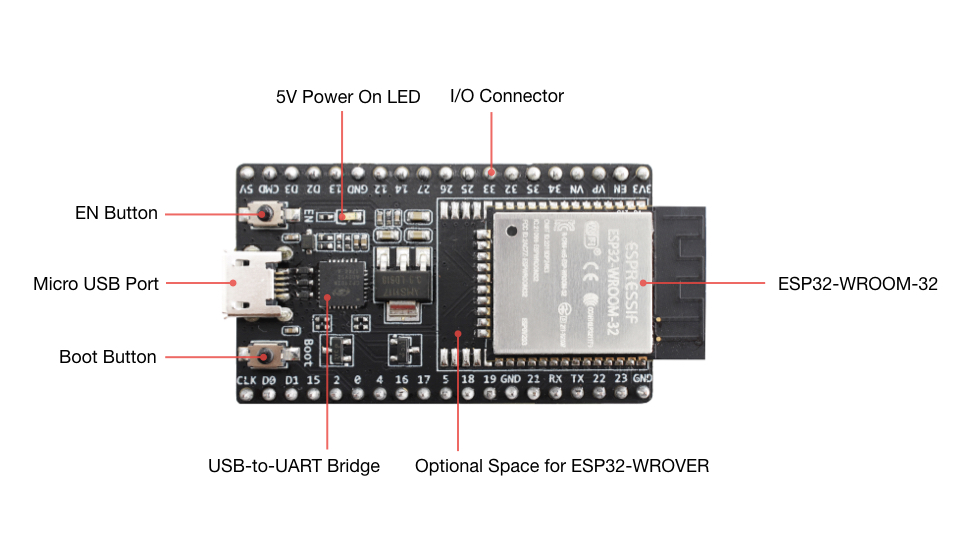
\includegraphics[scale=0.4]{images/esp32-devkitc.jpg}
    %    \caption{ESP32-DevKitC V4 with ESP32-WROOM-32 module
    %        \cite{esp32-gettingStarted_w}}
    %    \label{esp32_img}
    %\end{figure}

%%%%%%%%%%%%%%%%%%%%%%%%%%%%%%%%%%%%%%%%%%%%%%%%%%%%%%%%%%%%%%%%%%%%%%%%%%%%%%%
\section{Environnement de développement}
    Trois environnements s'offrent à nous:
    \begin{enumerate}
        \item \textbf{MicroPython}\\
            Selon le site officiel de MicroPython\cite{micropython_w}, MicroPython
            est une implémentation simple et efficace de Python 3 incluant un
            petit sous-ensemble de la bibliothèque standard Python et est
            optimisé pour fonctionner sur des microcontrôleurs.\\
            MicroPython est open source et facile à utiliser. Cependant,
            il n'est pas assez bas niveau pour ce projet.\\
            Par exemple il serait impossible d'envoyer des paquets au niveau de la
            couche lisaison de données ou encore, avoir accès aux tables de routages \textsc{ip}.\\
        
        \item \textbf{IoT Development Framework (IDF)}\\
            IDF est l'environnement du constucteur de l'\esp\ (Espressif).
            La documentation est complète mais le code source n'est pas entièrement
            disponible. Pour certaines parties du framework, nous n'avons accès qu'aux
            fichiers d'entête.\\
            Ce framework est natif et nous apportera donc une plus grande fidélité à l'\esp. \\
            Cet environnement nous donne aussi accès à des fonctionnalités de FreeRTOS
            (free real-time operating system).\\
            FreeRTOS est un système d'exploitation temps réel open source pour microcontrôleurs.
            Ses fonctionnalités pourront nous être utiles pour le projet.\\

        \item \textbf{Arduino}\\
            L'environnement Arduino se base sur IDF. Il est donc possible que certaines
            fonctionnalités d'IDF ne soient pas disponible. 
            La documentation est moins complète qu'IDF mais tout le code source est disponible.
            Cet environnement semble assez bas niveau car nous avons accès au driver Ethernet
            et à la couche \textsc{ip}.
    \end{enumerate}
    \vspace{1cm}
    Il est évident que nous ne choisirons pas MicroPython car certaines fonctionnalités utiles
    pour ce projet ne sont pas accessibles.\\
    Nous choisirons IDF pour sa documentation complète, sa nativité et l'accès aux
    fonctionnalités de FreeRTOS.

%%%%%%%%%%%%%%%%%%%%%%%%%%%%%%%%%%%%%%%%%%%%%%%%%%%%%%%%%%%%%%%%%%%%%%%%%%%%%%%
\section{Protocoles de routage}
    Dans cette section, nous discutons des différents protocoles de routage envisageables.\\
    Nous allons d'abord établir un classement des protocoles de routage \mesh.\\
    Ensuite nous allons décrire brièvement les protocoles les plus cités dans la littérature pour les classer
    en fonction de leur appartenance à une catégorie établie dans notre classement. 
    Enfin, nous pourrons choisir un protocole à implémenter pour ce projet.\\

    \underline{\textbf{Classification}}\\

    Les protocoles de routages \mesh\ peuvent être divisés en deux grandes catégories:
    \begin{enumerate}
        \item \textbf{Proactifs}: Les noeuds maintiennent une/des table(s) de routage
            qui stockent les routes vers tous les noeuds du réseau. 
            Ils envoient régulièrement des paquets de contrôle à travers le réseau pour échanger et 
            mettre à jour l'information de leurs voisins.
        \item \textbf{Réactifs}: Ces protocoles établissent une route uniquement quand des paquets
            doivent être transférés.
    \end{enumerate}
    Nous écarterons les protocoles proactifs pour ce projet car ils gardent
    beaucoup d'information en mémoire. Ils ne passent donc pas à l'échelle.\\
    Les protocoles réactifs sont plus économes en ressources mais nécessitent parfois un délai
    plus long pour établir une route
    car elles sont établies à la demande.\\

    \underline{\textbf{Description}}\\

    Il existe une multitude de protocols de routage \mesh.
    Ci-dessous, en voici quelques-uns souvent cités dans la littérature:\\
    \begin{itemize}
        \item \textbf{AODV}\cite{aodv_w} Ad-hoc On-demand Distance Vector\\
            Protocole réactif à vecteur de distance que nous décrirons en détail par la suite.\\
        \item \textbf{DSR}\cite{dsr_w} Dynamic Source Routing\\
            Similaire à AODV mais ici, les paquets servant à la découverte d'un chemin
            (\textit{RREQ}) contiennent tous les sauts de ce chemin.\\
        \item \textbf{OLSR}\cite{olsr_w} Optimized Link State Routing\\
            Protocole proactif à état de liens. Dans ce protocole, certains noeuds servent de relais pour effectuer
            le broadcasting des paquets servant à la découverte de chemins. L'ensemble de ces noeuds forme un arbre couvrant du réseau.\\
        \item \textbf{B.A.T.M.A.N}\cite{batman_w} Better Approach to Mobile Adhoc Networking\\
            Protocole proactif à état de liens. Le protocole ne calcule
            pas le chemin pour atteindre un noeud mais le meilleur saut dans la bonne direction.
            Pour cela, pour chaque destination il va sélectionner son voisin qui lui a transmis
            le plus de messages de cette destination.\\
        \item \textbf{DSDV}\cite{dsdv_w} Destination Sequence Distance Vector\\
            Protocole à vecteur de distance basé sur l'algorithme de Bellman-Ford.
    \end{itemize}

    Nous pouvons donc classer ces protocoles de la manière suivante: 
    \begin{diagram}[H]
        \Tree[.{wireless network protocols} 
            [.Reactive [.\textsc{aodv} ]
                [.\textsc{dsr} ]]
            [.Proactive [.{Link-state} 
                [.\textsc{olsr} ] 
                [.\textsc{b.a.t.m.a.n} ]] 
                [.{Distance-vector} [.\textsc{dsdv} ]]]]
        \caption{Classifications des protocols de routage }
    \end{diagram}

    \underline{\textbf{Choix d'un protocole}}\\

    Comme dit plus haut, nous écartons les protocoles proactifs. Il nous reste donc le choix entre \aodv\ et \textsc{dsr}.
    Nous allons retenir \aodv\ pour la taille fixe de ses paquets. En effet, \textsc{dsr} utilise plus de données quand
    les routes contiennent un grand nombre de sauts.

    
    
%    Dans cette section nous discutons de différents protocoles de routage envisageables.\\
%    Tout d'abord, nous établirons un classement des différents types de protocoles de routage\mesh. \\
%    Ensuite, nous etudierons et comparerons différents protocoles de routage mesh: \espmesh\
%    \cite{esp-mesh_w}, OLSR\cite{olsr_w}, AODV\cite{aodv_w} et DSR\cite{dsr_w}\\
%    Enfin nous allons choisir un protocole à implémenter sur \esp.\\
%    
%    \subsection{Classification}
%    Les protocoles de routages \mesh\ peuvent être divisés en deux grandes catégories:
%    \begin{enumerate}
%        \item \textbf{Proactifs}: Les noeuds maintiennent une/des table(s) de routage
%            qui stockent les routes vers tous les noeuds du réseau. 
%            Ils envoient régulièrement des paquets de contrôle à travers le réseau pour échanger et 
%            mettre à jour l'information de leurs voisins.
%        \item \textbf{Réactifs}: Ces protocoles établissent une route uniquement quand des paquets
%            doivent être transférés.
%    \end{enumerate}
%    Nous écarterons les protocoles proactifs pour ce projet car ils gardent
%    beaucoup d'information en mémoire. Ils ne passent donc pas à l'échelle.\\
%    Les protocoles réactifs sont plus économes en ressources mais nécessitent parfois un délai
%    plus long pour établir une route
%    car elles sont établies à la demande.\\
%    
%    Il existe une multitude de protocols de routage \mesh. 
%    Ci-dessous, en voici quelques-uns souvent cités dans la littérature:\\
%    \begin{itemize}
%        \item \textbf{AODV}\cite{aodv_w} Ad-hoc On-demand Distance Vector\\
%            Protocole réactif à vecteur de distance que nous décrirons en détail par la suite.\\
%        \item \textbf{DSR}\cite{dsr_w} Dynamic Source Routing\\
%            Similaire à AODV mais ici, les paquets servant à la découverte d'un chemin
%            (\textit{RREQ}) contiennent tous les sauts de ce chemin.\\
%        \item \textbf{OLSR}\cite{olsr_w} Optimized Link State Routing\\
%            Protocole proactif à état de liens. Dans ce protocole, certains noeuds servent de relais pour effectuer
%            le broadcasting des paquets servant à la découverte de chemins. L'ensemble de ces noeuds forme un arbre couvrant du réseau.\\
%        \item \textbf{B.A.T.M.A.N}\cite{batman_w} Better Approach to Mobile Adhoc Networking\\
%            Protocole proactif à état de liens. Le protocole ne calcule
%            pas le chemin pour atteindre un noeud mais le meilleur saut dans la bonne direction.
%            Pour cela, pour chaque destination il va sélectionner son voisin qui lui a transmis
%            le plus de messages de cette destination.\\
%        \item \textbf{DSDV}\cite{dsdv_w} Destination Sequence Distance Vector\\
%            Protocole à vecteur de distance basé sur l'algorithme de Bellman-Ford.
%    \end{itemize}
%    On peut donc classer ces protocoles de la manière suivante: 
%    \begin{diagram}[H]
%        \Tree[.{wireless network protocols} 
%            [.Reactive [.\textsc{aodv} ]
%                [.\textsc{dsr} ]]
%            [.Proactive [.{Link-state} 
%                [.\textsc{olsr} ] 
%                [.\textsc{b.a.t.m.a.n} ]] 
%                [.{Distance-vector} [.\textsc{dsdv} ]]]]
%        \caption{Classifications des protocols de routage }
%    \end{diagram}
%
%
%%%%%%%%%%%%%%%%%%%%%%%%%%%%%%%%%%%%%%%%%%%%%%%%%%%%%%%%%%%%%%%%%%%%%%%%%%%%%%%
%\chapter{ESP MESH}
        \espmesh\ est le protocole du constructeur Espressif permettant d'établir un réseau mesh avec des \esp.
        Cette section explique le fonctionnement de ce protocole. \espmesh\ a pour objectif la création d'un arbre recouvrant.
        Il existe plusieurs types de noeuds:
        \begin{enumerate}
            \item \textbf{Racine}: seule interface entre le réseau \espmesh\ et un réseau \textsc{ip} externe.
            \item \textbf{Noeuds intermédiaires}: noeuds qui ont un parent et au moins un enfant.
            Ils transmettent leurs paquets et ceux de leurs enfants.
            \item \textbf{Feuilles}: noeuds qui n'ont pas d'enfants et ne transmettent que leurs paquets.
            \item \textbf{Noeuds idle}: noeuds qui n'ont pas encore rejoint un réseau \espmesh.
        \end{enumerate}

        \begin{figure}[H]
            \centering
            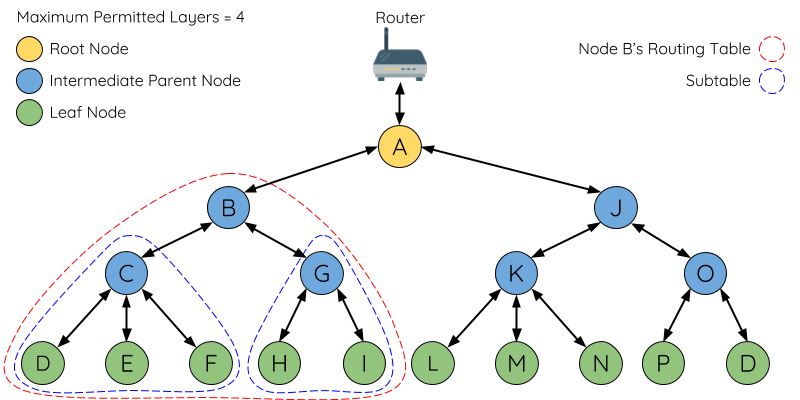
\includegraphics[scale=0.3]{images/mesh-node-types.png}
            \caption{Topologie d'un réseau \espmesh \cite{esp-mesh_w}}
        \end{figure}

        \textbf{Routage}\newline
        \begin{itemize}
            \item Table de routage\\
                Chaque noeud possède sa table de routage. Soit $p$ un noeud, sa table de routage contient les adresses \mac\ 
                des noeuds du sous-arbre ayant $p$ comme racine, et également celle de $p$.\\
                Elle est partitionnée en sous-tables qui correspondent aux sous-arbres des enfants de $p$.
                Par exemple, nous pouvons apercevoir sur la figure précédente, la table de routage du noeud B (en rouge).
                Elle est partitionnée en 2 sous-table (en bleu) contenant respectivement les noeuds C, D, E, F et G, H, I.
            \item Acheminement de paquets\\
                Quand un paquet est reçu,
                \begin{itemize}
                    \item Si l'adresse \mac\ du paquet est dans la table de routage et si elle est différente de l'adresse du noeud l'ayant reçu, le paquet est envoyé
                    à l'enfant correspondant à la sous-table contenant l'adresse.
                    \item Si l'adresse n'est pas dans la table de routage, le paquet est envoyé au parent.
                \end{itemize}
                %\espmesh\ utilise un mécanisme de vérification de chemin pour détecter les boucles. Si une boucle arrive, un parent va prévenir son enfant et initier une déconnexion.

        \end{itemize}
        \vspace{0.5cm}

        \textbf{Construction d'un réseau}
        \newline
        \begin{enumerate}
            \item \'Election de la racine
                \begin{itemize}
                    \item \textbf{Sélection automatique}\\
                        Chaque noeud idle va transmettre son adresse \mac\ et
                        la valeur de son \rssi\ (Received Signal Strength Indication) avec le routeur via des beacons.
                        Dans le but de choisir comme racine, le noeud le plus proche de l'AP.
                        Simultanément, chaque noeud scanne les beacons des autres noeuds. Si un noeud
                        en détecte un autre avec un \rssi\ strictement plus fort, il va transmettre le contenu de
                        ce beacon (càd voter pour ce noeud).
                        Ce processus sera répété pendant un nombre minimum d'itérations (10 par défaut).
                        Une itération pour un noeud, consiste à avoir reçu les beacons de tous les autres noeuds
                        et avoir voté pour le noeud ayant le meilleur \rssi\ avec le routeur.
                        Après toutes les itérations, chaque noeud va calculer le ratio suivant: 
                        \[\frac{nombre\ de\ votes\ pour\ ce\ noeud}{nombre\ de\ noeuds\ participants\ \textrm{\textit{à l'élection}}}\]
                        Cest deux informations sont connues par la réception des beacons.
                        Si ce ratio est au-dessus d'un certain seuil (par défaut 90\%), ce noeud deviendra la racine.\footnote{
                            Si plusieurs racines sont élues, deux réseaux \espmesh\ seront créés.
                            Dans ce cas, \espmesh\ possède un mécanisme interne (dont le fonctionnement n'est pas décrit par Espressif) qui va fusionner les deux réseaux
                            ssi les racines sont connectées au même routeur.
                        }



                    \item \textbf{Sélection par l'utilisateur}\\
                        Le choix de la racine peut être réalisé par l'utilisateur via l'\textsc{API} \espmesh.
                        Dans ce cas, la racine se connecte au routeur et elle, ainsi que les autres noeuds, oublient le processus
                        d'élection.
                \end{itemize}
            \item Formation de la deuxième couche\\
                %Une fois le processus d'élection d'une racine terminé, chaque noeud va émettre des beacons
                %pour permettre aux autres noeuds de détecter sa présence et de connaître son statut.
                %Ces beacons contiennent les informations suivantes:
                %\begin{itemize}
                %    \item[$\bullet$] Type du noeud (racine, intermédiaire, feuille, idle)
                %    \item[$\bullet$] Couche sur laquelle se trouve le noeud
                %    \item[$\bullet$] Nombre de couches maximum autorisées dans le réseau
                %    \item[$\bullet$] Nombre de noeuds enfants
                %    \item[$\bullet$] Nombre maximum d'enfants   
                %\end{itemize}
                %Les noeuds idle à portée de la racine vont s'y connecter et devenir des noeuds intermédiaires.
                Une fois le processus d'élection d'une racine terminé,
                les noeuds idle à portée de la racine vont s'y connecter et devenir des noeuds intermédiaires
            
            \item Formation des autres couches\\
                %Les noeuds idle à portée de noeuds intermédiaires vont s'y connecter. 
                Chaque noeud du réseau \espmesh\ émet périodiquement des beacons contenant les
                informations suivantes:
                \begin{itemize}
                    \item[$\bullet$] Type du noeud (racine, intermédiaire, feuille, idle)
                    \item[$\bullet$] Couche sur laquelle se trouve le noeud
                    \item[$\bullet$] Nombre de couches maximum autorisées dans le réseau
                    \item[$\bullet$] Nombre de noeuds enfants
                    \item[$\bullet$] Nombre maximum d'enfants   
                \end{itemize}
                %Sur base de ces beacons, les noeuds idle vont connaître leurs potentiels parents. Si plusieurs parents
                %sont possibles, un noeud choisira son parent selon deux critères connus par les beacons des noeuds intermédiaires.
                Sur base du contenu de ces beacons, les noeuds idle conaissent leurs potientiels parents.
                Si plusieurs parents sont possibles, un noeud choisira son parent selon deux critères:
                \begin{enumerate}
                    \addtolength{\itemindent}{1cm}
                    \item[1.] La couche sur laquelle se situe le candidat parent:
                        le candidat se trouvant sur la couche la moins profonde sera choisi. 
                    \item[2.] Le nombre d'enfants du candidat parent: si plusieurs candidats se trouvent
                        sur la couche la moins profonde, celui avec le moins d'enfants sera choisi. 
                \end{enumerate}
                
                Un noeud peut également se connecter à un parent prédéfini.
                Une fois connectés, les noeuds deviennent des noeuds intermédiaires si le nombre maximal de couches n'est pas atteint.
                Sinon, les noeuds de la dernière couche deviennent automatiquement
                des feuilles, empêchant d'autres noeuds dans l'état idle de s'y connecter.

        \end{enumerate}
        Pour éviter les boucles, un noeud ne va pas se connecter à un noeud dont l'adresse \mac\ se trouve dans sa table de routage.
        \vspace{0.5cm}\\
        \textbf{Mise sous tension asynchrone}\newline
            La structure du réseau peut être affectée par l'ordre dans lequel les noeuds sont mis sous tension.
            Les noeuds ayant une mise en tension retardée suivront les deux règles suivantes:
            \begin{enumerate}
                \item Si le noeud détecte, par les beacons, qu'une racine existe déjà, il ne vas pas essayer
                    d'élire une nouvelle racine
                    même si son \rssi\ avec le routeur est meilleur. Il va rejoindre le réseau comme un noeud idle. \\
                    Si le noeud est la racine désignée, tous les autres noeuds vont rester idle
                    jusqu'à ce que le noeud soit mis sous tension.
                \item Si le noeud devient un noeud intermédiraire, il peut devenir le meilleur parent d'un autre noeud 
                (cet autre noeud changera donc de parent).
                \item Si un noeud idle a un parent prédéfini et que ce noeud n'est pas sous tension, il ne va pas essayer
                de se connecter à un autre parent.
            \end{enumerate}
        \vspace{0.5cm}
        \textbf{Défaillance d'un noeud}\newline
            \begin{itemize}
                \item Défaillance de la racine\\
                    Si la racine tombe, les noeuds de la deuxième couche vont d'abord tenter de s'y reconnecter.
                    Après plusieurs échecs, les noeuds de la deuxième couche vont entamer entre eux le processus d'élection d'une nouvelle racine.
                    Si la racine ainsi que plusieurs couches tombent, le processus d'élection sera initialisé sur la couche la plus haute.


                \item Défaillance d'un noeud intermédiaire\\
                    Si un noeud intermédiaire tombe, ses enfants vont d'abord tenter de s'y reconnecter.
                    Après plusieurs échecs, ils se connecteront au meilleur parent disponible.
                    S'il n'y a aucun parent possible, ils se mettront dans l'état idle.
                    \begin{figure}[H]
                        \centering
                        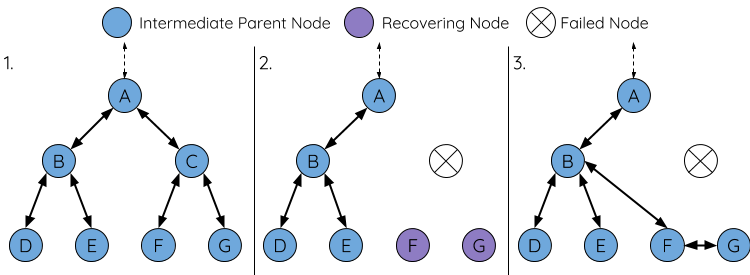
\includegraphics[scale=0.5]{images/mesh-parent-node-failure.png}
                        \caption{Défaillance d'un noeud intermédiaire\cite{esp-mesh_w}}
                    \end{figure}
            \end{itemize}
            \vspace{0.5cm}
            \textbf{Changement de racine}\newline
                Un changement de racine n'est possible que dans deux situations:
                \begin{enumerate}
                    \item La racine tombe. (voir point précédent)
                    \item La racine le demande via un appel à \textbf{esp\_mesh\_waive\_root()}.
                        Dans ce cas, un processus d'élection de racine sera initialisé. La nouvelle racine élue
                        enverra alors une \textit{switch request} à la racine actuelle qui répondra par un acquittement.
                        Ensuite la nouvelle racine se déconnectera de son parent et se connectera au routeur.
                        L'ancienne racine se déconnectera du routeur et deviendra un noeud idle pour enfin se connecter à un nouveau parent.
                \end{enumerate}
        \textbf{Paquets ESP-MESH}\\
            Les paquets \espmesh\ sont contenus dans une trame \wifi. Une transmission multi-sauts utilisera un paquet \espmesh\ transporté 
            entre chaque noeud par une trame \wifi\ différente.
            La figure \ref{fig_meshPacket} montre la structure d'un paquet \espmesh:\\

            \begin{figure}[h]
                \centering
                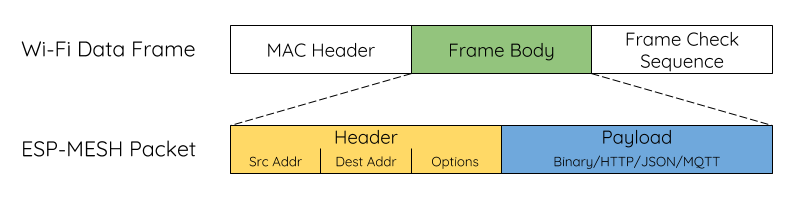
\includegraphics[scale=0.5]{images/mesh-packet.png}
                \caption{Paquet \espmesh\ \cite{esp-mesh_w}}
                \label{fig_meshPacket}
            \end{figure}
            Le header d'un paquet \espmesh\ contient les adresses source et destination ainsi que diverses options.
            Le payload d'un paquet \espmesh\ contient les données de l'application.

            Dans le cas où l'adresse de destination est une adrese \textsc{ip}, le paquet sera envoyé à la racine du réseau
            \espmesh\ qui transmet le payload du paquet (par exemple en initiant une connexion tcp avec un socket).
        \vspace{0.5cm}\\
        \textbf{Contrôle de flux}\\
            Pour éviter que les parents soient submergés de flux venant de leurs enfants, chaque parent va
            assigner une fenêtre de réception à chaque enfant. Chaque noeud enfant doit demander une fenêtre
            de réception avant chaque transmission. La taille de la fenêtre peut être ajustée dynamiquement.
            Une transmission d'un enfant vers un parent se déroule en plusieurs étapes:
            \begin{enumerate}
                \item Le noeud enfant envoit à son parent une requête de fenêtre. Cette requête contient le numéro de séquence du paquet en attente d'envoi.
                \item Le parent reçoit la requête et compare le numéro de séquence avec celui du précédent paquet envoyé par l'enfant.
                    La comparaison est utilisée pour calculer la taille de la fenêtre qui est transmise à l'enfant.\footnote{Ce calcul n'est pas précisé par Espressif}
                \item L'enfant transmet le paquet conformément à la taille de fenêtre spécifiée par le parent. Une fois la fenêtre de réception utilisée, l'enfant doit renvoyer une demande de fenêtre.
            \end{enumerate}
        \vspace{0.5cm}
        \textbf{Performances}\\
            Espressif fournit les performances d'\espmesh\ pour un réseau de maximum 100 noeuds, 6 couches et
            un nombre d'enfants par noeud de 6 (voir table \ref{performances_espMesh}).
            \begin{table}[H]
                \begin{tabular}{|l|l|}
                    \hline
                    Temps de construction du réseau & $<$ 60 secondes\\ \hline
                    Latence par saut & 10 à 30 millisecondes\\ \hline
                    Temps de réparation du réseau & \makecell{Si la racine tombe: $<$ 10 secondes \\ Si un noeud enfant tombe: $<$ 5 secondes}\\ \hline
                \end{tabular}
                \caption{Performances d'\espmesh\ \cite{esp-mesh_w}}
                \label{performances_espMesh}
            \end{table}
            \hspace{-0.75cm}
            \textbf{Discussion}\\
            A première vue, une topologie en arbre n'est pas robuste car si la racine tombe,
            tout le reste du réseau est déconnecté. Cependant le processus d'élection
            d'une nouvelle racine semble efficace selon les résulats fournis par Espressif.
            Un point négatif du protocole est que pour un noeud donné, sa table de routage contient tous les
            noeuds de son sous-arbre.
            On imagine donc difficilement utiliser ce protocole pour un nombre élevé de noeuds.    
%    \vspace{1cm}
%%%%%%%%%%%%%%%%%%%%%%%%%%%%%%%%%%%%%%%%%%%%%%%%%%%%%%%%%%%%%%%%%%%%%%%%%%%%%%% 
%\newpage 
%\chapter{AODV}
    Ad-hoc On-demand Distance Vector (\aodv) est un protocole réactif à vecteur de distance.
    Les 3 types de messages définis dans \aodv\ sont les Route requests (\textit{\rreq s}),
    les Route Remplies (\textit{\rrep s}) et les Route Errors (\textit{\rerr s}).
    Comme illustré sur la figure suivante, le premier sera envoyé en flooding par un noeud
    désirant obtenir une nouvelle route pour
    une desination donnée. Le second sert de réponse au premier. Il est envoyé à l'émetteur du
    \rreq. Et le dernier sert notamment lorsqu'un lien d'une route active est brisé. 
    Nous détaillons plus bas ces mécanismes.
    \vspace{1cm}
    \begin{figure}[H]
        \centering
        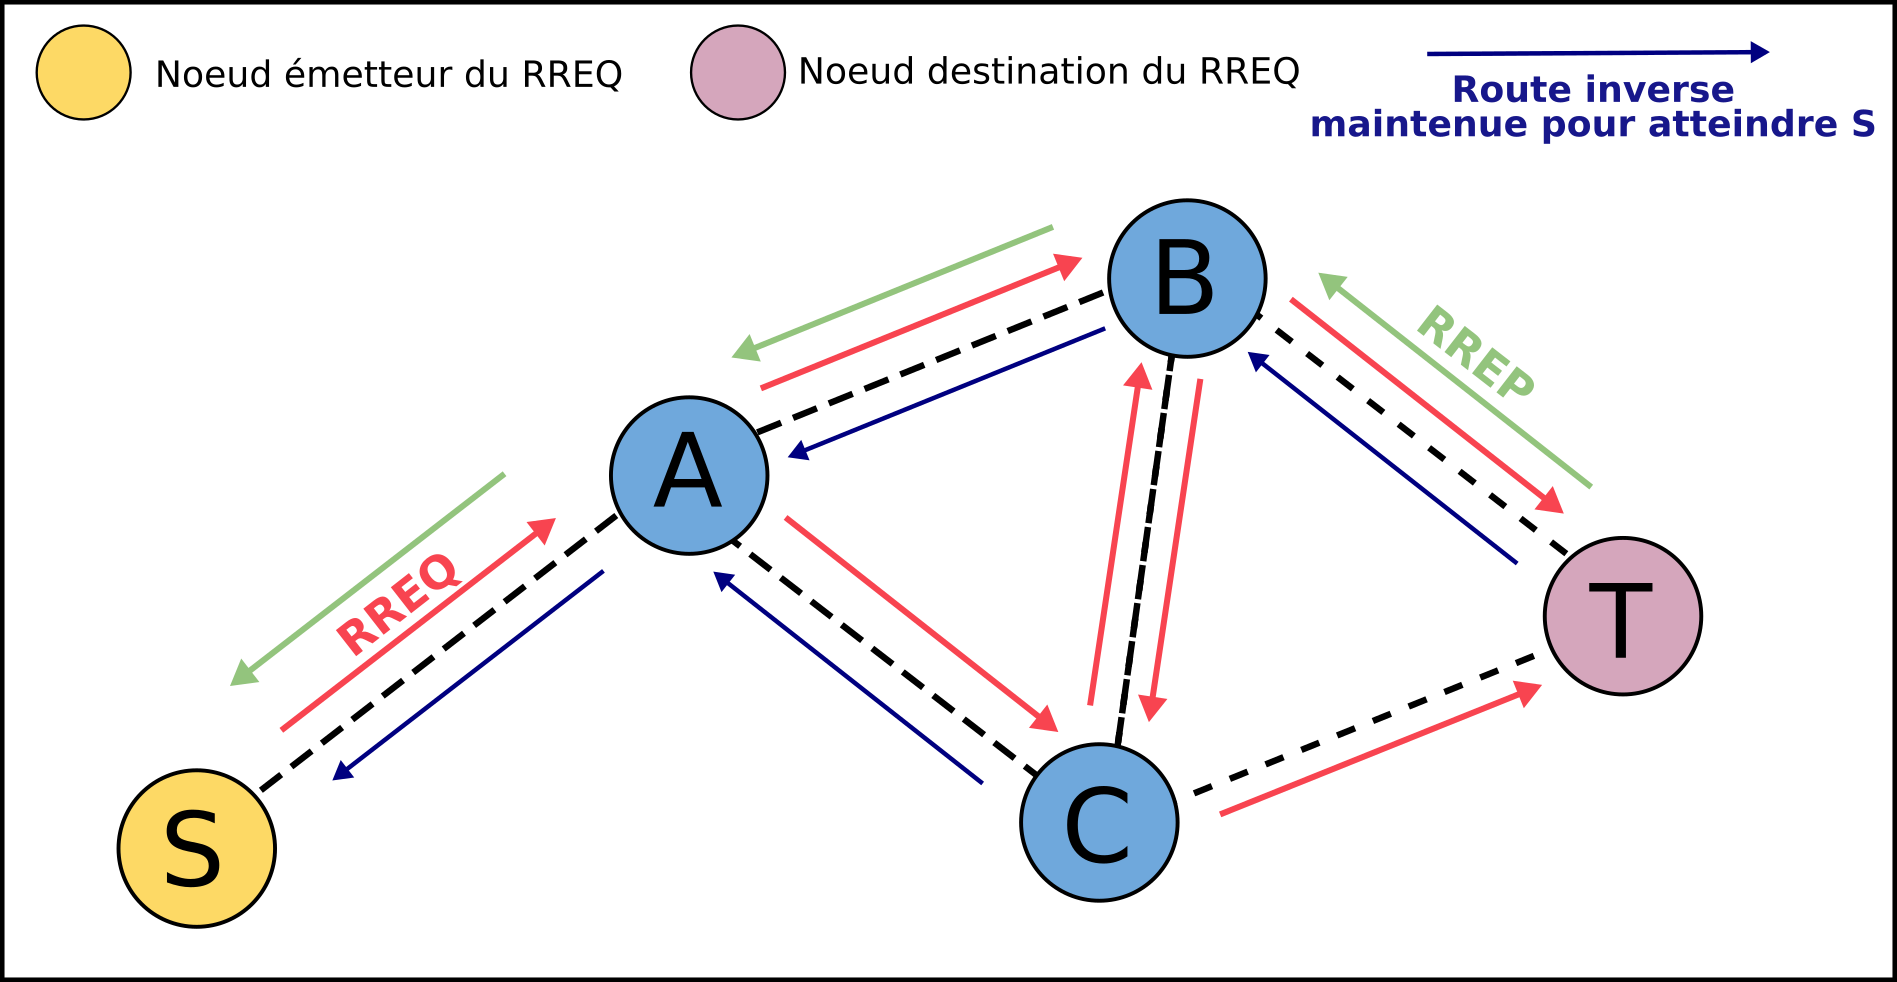
\includegraphics[scale=0.35]{images/aodv.png}
        \caption{Illusration du fonctionnement d'AODV}
        \label{aodv}
    \end{figure}
    
    
    \vspace{0.5cm}
    %\textbf{Format des paquets}\\
    \section{Format des paquets}
        \textbf{RREQ}\\
            \begin{figure}[H]
                \centering
                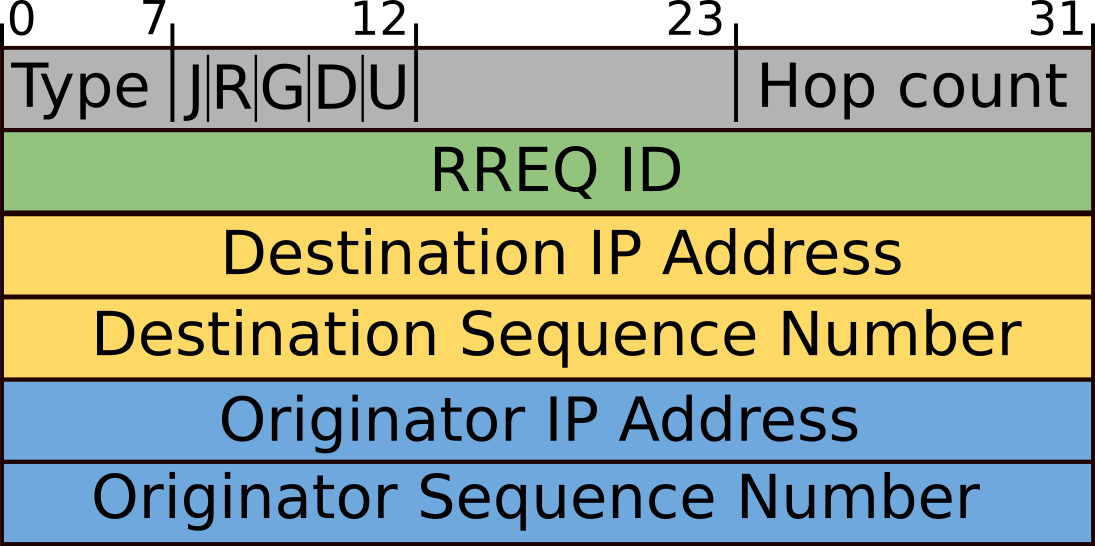
\includegraphics[scale=0.5]{images/rreq.png}
                \caption{Format d'un paquet \rreq\ \cite{rfc_aodv}}
                \label{rreqPaquet}
            \end{figure}
            Le format d'un \rreq\ est illustré sur la figure précédente. Il contient les champs
            repris dans la table suivante:\\
            \begin{table}[H]
                \begin{tabular}{ll}
                    type & \makecell[l]{$=1$}\\\hline
                    J R G & \makecell[l]{flags}\\\hline
                    D  & \makecell[l]{flag indiquant que seul la destination peut\\ répondre au \rreq}\\\hline
                    U & \makecell[l]{flag indiquant que le numéro de séquence de la\\ destination est inconnu}\\\hline
                    Hop count & \makecell[l]{nombre de sauts depuis le noeud source}\\\hline
                    \rreq\ \textsc{id} & \makecell[l]{numéro de séquence identifiant le \rreq}\\\hline
                    Destination IP Address & \makecell[l]{adresse \textsc{ip} du noeud pour lequel la route\\ est demandée}\\\hline
                    Destination Sequence Number & \makecell[l]{le dernier numéro de séquence connu pour une \\route vers la destination}\\\hline
                    Originator IP Address & \makecell[l]{adresse ip de l'émetteur du \rreq}\\\hline
                    Originator Sequence Number & \makecell[l]{numéro de séquence à utiliser pour une route\\ pointant vers l'émetteur du \rreq}\\
                \end{tabular}
                \caption{Champs d'un \rreq\ \cite{rfc_aodv}}
                \label{rreq_fields}
            \end{table}
            
        \textbf{RREP}\\
            \begin{figure}[H]
                \centering
                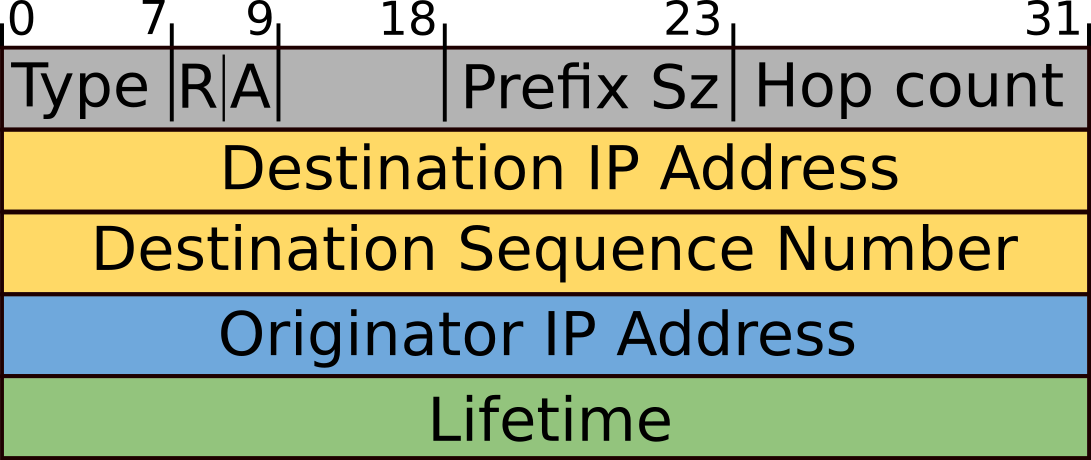
\includegraphics[scale=0.5]{images/rrep.png}
                \caption{Format d'un \rrep\ \cite{rfc_aodv}}
                \label{rreqPaquet}
            \end{figure}
            Le format d'un \rrep\ est illustré sur la figure précédente. Il contient les champs
            repris dans la table suivante:\\
            \begin{table}[H]
                \begin{tabular}{ll}
                    type & \makecell[l]{$=2$}\\ \hline
                    R & \makecell[l]{flag utilisé pour le multicast}\\ \hline
                    Prefix size & \makecell[l]{utilisé pour les aggrégations de routes}\\ \hline
                    Hop Count & \makecell[l]{nombre de sauts de l'\textit{originator} à la destination}\\ \hline
                    Destination IP address & \makecell[l]{adresse IP de du noeud pour qui l'adresse \\est demandée}\\ \hline
                    Destination Sequence Number & \makecell[l]{numéro de séquence de destination \\associé à la route}\\ \hline
                    Originator IP address & \makecell[l]{adresse IP du noeud émetteur du \rreq}\\ \hline
                    Lifetime & \makecell[l]{temps (en ms) pendant lequel le noeud qui reçoit \\le \rrep\ va considérer la route valide}\\
                \end{tabular}
                \caption{Champs d'un \rrep\ \cite{rfc_aodv}}
                \label{rrep_fields}
            \end{table}

    %\textbf{Découverte d'un chemin}\\
    \section{Découverte d'un chemin}
        La découverte d'un chemin est intiée par un noeud voulant envoyer des paquets à une destination pour laquelle il n'a aucune route valide.
        Chaque noeud possède deux compteurs: \textit{sequence\_number} et \textit{rreq\_id}.
        
        
        \vspace{0.5cm}
        \textbf{Génération du RREQ}\\
            Le noeud source incrémente ses compteurs \textit{sequence\_number} et \textit{rreq\_id} de 1.
            Il envoie ensuite un \rreq\ en broadcast à ses voisins.
        
        
        \vspace{0.5cm}
        \textbf{Propagation du RREQ}\\
            \begin{itemize}
                \item[$\bullet$] Noeud intermédiaire\\
                    A la réception d'un \rreq, un noeud intermédiaire va pouvoir rajouter ou mettre à jour
                    les routes vers son prédécesseur et vers le noeud source du \rreq.\\
                    Ensuite deux situations sont possibles:
                    \begin{enumerate}
                        \item Le noeud courant possède une route active vers la destination et le numéro de séquence de la route est plus grand 
                            ou égal au numéro de séquence de la destination dans le \rreq.
                            Dans ce cas, il peut envoyer par unicast un \rrep\ à la source du \rreq.
                        \item Sinon\\
                            Le noeud va incrémenter le nombre de sauts du \rreq\ et le propager à ses voisins.
                    \end{enumerate}

                \item[$\bullet$] Noeud destination\\
                    A la réception d'un \rreq\  lui étant destiné, un noeud va, comme un noeud intermédiaire, 
                    rajouter ou mettre à jour les routes vers son prédécesseur et vers le noeud source du \rreq.
                    Si le \textit{Destination Sequence Number} du \rreq\ est égal à son \textit{sequence\_number},
                    il va incrémenter ce dernier et envoyer un \rrep\ en unicast vers la source du \rreq.     
            \end{itemize}

        \vspace{0.5cm}
        \textbf{Propagation du RREP}\\
            A la réception d'un \rrep\ , un noeud va pouvoir rajouter ou mettre à jour
            les routes vers le noeud source du \rrep\  et vers son successeur.\\
            Il va ensuite incrémenter le nombre de sauts du \rrep\  et le propager en unicast vers la destination de ce \rrep\ .
            Cette propagation en unicast vers la source du \rreq\ est possible par l'apprentissage de la route inverse
            (destination du \rreq\ vers l'émetteur du \rreq) réalisée lors du flooding du \rreq.

    %\underline{\textbf{Table de routage}}\\
    \section{Table de routage}
        Chaque entrée d'une table de routage contient les informations suivantes:
        
        \begin{table}[H]
            \centering
            \begin{tabular}{|l|l|}
                \hline
                \textit{dest}       & Adresse IP de destination\\
                \textit{dest\_SN}   & Numéro de séquence de destination\\
                \textit{flag}       & Indicateur de numéro de séquence de destination valide\\
                \textit{out}        & Interface réseau\\
                \textit{hops}       & \makecell[l]{Comptage de sauts (nombre de sauts nécessaires\\ pour atteindre la destination)}\\
                \textit{next-hop}   & Prochain saut\\
                \textit{precursors} & Liste des précurseurs\\
                \textit{lifetime}   & temps d'expiration ou de suppression de l'itinéraire\\
                \hline
            \end{tabular}
            \caption{entrée d'une table de routage \aodv \cite{rfc_aodv}}
            \label{routingTable_aodv}
        \end{table}

        \textbf{Mise à jour de la table de routage}\\
            Soit N une nouvelle route et O la route existante.\\
            O est mise à jour si:\\
            \begin{center}
                \begin{tabular}{|l|}
                    \hline
                    $O.SN \leq N.SN$ \\
                    \textbf{ou} ($O.SN = N.SN$ \textbf{et} $O.hop\_count > N.hop\_count$)\\
                    \hline
                \end{tabular}
            \end{center}
        
        \textbf{Gestion du \textit{lifetime}}\\
            Le temps de vie d'une route dans la table de routage est initialisé à \textit{active\_route\_timeout} (3 millisecondes).\\
            Quand ce timer expire, la route passe de active à inactive. Une route inactive ne pourra plus être utilisée pour transférer des données
            mais pourra fournir des informations pour de futurs \rreq\  et la réparation de routes.\\
            Quand une route est utilisée, son temps de vie  est actualisé à: $current time + active\_route\_timeout$

    %\vspace{0.5cm}
    %\textbf{Evitement de boucles}\\
    \section{Evitement de boucles}
        A priori les numéros de séquences suffisent pour éviter les boucles. Cependant, d'après \cite{loop_aodv}, il y a des
        ambiguités dans le RFC \cite{rfc_aodv}. Dû à ces ambiguités, l'implémentation pourrait introduire des boucles.
        %Certaines parties du RFC concerant la gestion des numéros de séquences pourraient introduiredes boucles. 
        Nous approfondirons la lecture de cet article si nous choisissons ce protocole afin d'éviter les boucles dans notre implémentation.

        %\vspace{0.5cm}
    %\textbf{Défaillance d'un lien}\\
    \section{Défaillance d'un lien}
        Un noeud faisant partie d'une route active broadcast des messages \textit{hello} (\rrep)
        régulièrement.\\
        Si un noeud ne reçoit pas de message durant un certain temps pour un voisin, il va considérer
        que le lien avec ce voisin est perdu.\\
        Dans ce cas, il va en informé ses voisins impactés par un \textsc{rerr}.
    
    \section{Discussion}
        Ce protocole semble plus robuste que \espmesh. Car en comparaison avec ce dernier, si un noeud tombe,
        les noeuds peuvent trouver une autre route pour envoyer des pauqtes d'un point à un autre.
        A priori cette robustesse dépend également de certains paramètre comme le temps de vie ou la fréquence
        d'émission des messages \textit{hello}.
        

\chapter{ESP MESH}
        \espmesh\ est le protocole du constructeur Espressif permettant d'établir un réseau mesh avec des \esp.
        Cette section explique le fonctionnement de ce protocole. \espmesh\ a pour objectif la création d'un arbre recouvrant.
        Il existe plusieurs types de noeuds:
        \begin{enumerate}
            \item \textbf{Racine}: seule interface entre le réseau \espmesh\ et un réseau \textsc{ip} externe.
            \item \textbf{Noeuds intermédiaires}: noeuds qui ont un parent et au moins un enfant.
            Ils transmettent leurs paquets et ceux de leurs enfants.
            \item \textbf{Feuilles}: noeuds qui n'ont pas d'enfants et ne transmettent que leurs paquets.
            \item \textbf{Noeuds idle}: noeuds qui n'ont pas encore rejoint un réseau \espmesh.
        \end{enumerate}

        \begin{figure}[H]
            \centering
            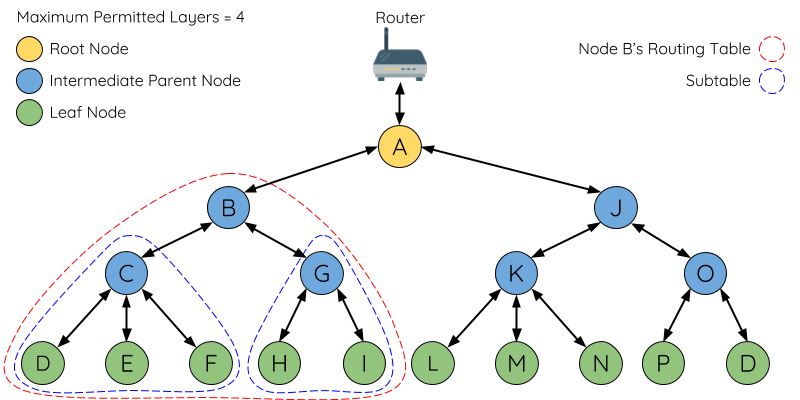
\includegraphics[scale=0.3]{images/mesh-node-types.png}
            \caption{Topologie d'un réseau \espmesh \cite{esp-mesh_w}}
        \end{figure}

        \textbf{Routage}\newline
        \begin{itemize}
            \item Table de routage\\
                Chaque noeud possède sa table de routage. Soit $p$ un noeud, sa table de routage contient les adresses \mac\ 
                des noeuds du sous-arbre ayant $p$ comme racine, et également celle de $p$.\\
                Elle est partitionnée en sous-tables qui correspondent aux sous-arbres des enfants de $p$.
                Par exemple, nous pouvons apercevoir sur la figure précédente, la table de routage du noeud B (en rouge).
                Elle est partitionnée en 2 sous-table (en bleu) contenant respectivement les noeuds C, D, E, F et G, H, I.
            \item Acheminement de paquets\\
                Quand un paquet est reçu,
                \begin{itemize}
                    \item Si l'adresse \mac\ du paquet est dans la table de routage et si elle est différente de l'adresse du noeud l'ayant reçu, le paquet est envoyé
                    à l'enfant correspondant à la sous-table contenant l'adresse.
                    \item Si l'adresse n'est pas dans la table de routage, le paquet est envoyé au parent.
                \end{itemize}
                %\espmesh\ utilise un mécanisme de vérification de chemin pour détecter les boucles. Si une boucle arrive, un parent va prévenir son enfant et initier une déconnexion.

        \end{itemize}
        \vspace{0.5cm}

        \textbf{Construction d'un réseau}
        \newline
        \begin{enumerate}
            \item \'Election de la racine
                \begin{itemize}
                    \item \textbf{Sélection automatique}\\
                        Chaque noeud idle va transmettre son adresse \mac\ et
                        la valeur de son \rssi\ (Received Signal Strength Indication) avec le routeur via des beacons.
                        Dans le but de choisir comme racine, le noeud le plus proche de l'AP.
                        Simultanément, chaque noeud scanne les beacons des autres noeuds. Si un noeud
                        en détecte un autre avec un \rssi\ strictement plus fort, il va transmettre le contenu de
                        ce beacon (càd voter pour ce noeud).
                        Ce processus sera répété pendant un nombre minimum d'itérations (10 par défaut).
                        Une itération pour un noeud, consiste à avoir reçu les beacons de tous les autres noeuds
                        et avoir voté pour le noeud ayant le meilleur \rssi\ avec le routeur.
                        Après toutes les itérations, chaque noeud va calculer le ratio suivant: 
                        \[\frac{nombre\ de\ votes\ pour\ ce\ noeud}{nombre\ de\ noeuds\ participants\ \textrm{\textit{à l'élection}}}\]
                        Cest deux informations sont connues par la réception des beacons.
                        Si ce ratio est au-dessus d'un certain seuil (par défaut 90\%), ce noeud deviendra la racine.\footnote{
                            Si plusieurs racines sont élues, deux réseaux \espmesh\ seront créés.
                            Dans ce cas, \espmesh\ possède un mécanisme interne (dont le fonctionnement n'est pas décrit par Espressif) qui va fusionner les deux réseaux
                            ssi les racines sont connectées au même routeur.
                        }



                    \item \textbf{Sélection par l'utilisateur}\\
                        Le choix de la racine peut être réalisé par l'utilisateur via l'\textsc{API} \espmesh.
                        Dans ce cas, la racine se connecte au routeur et elle, ainsi que les autres noeuds, oublient le processus
                        d'élection.
                \end{itemize}
            \item Formation de la deuxième couche\\
                %Une fois le processus d'élection d'une racine terminé, chaque noeud va émettre des beacons
                %pour permettre aux autres noeuds de détecter sa présence et de connaître son statut.
                %Ces beacons contiennent les informations suivantes:
                %\begin{itemize}
                %    \item[$\bullet$] Type du noeud (racine, intermédiaire, feuille, idle)
                %    \item[$\bullet$] Couche sur laquelle se trouve le noeud
                %    \item[$\bullet$] Nombre de couches maximum autorisées dans le réseau
                %    \item[$\bullet$] Nombre de noeuds enfants
                %    \item[$\bullet$] Nombre maximum d'enfants   
                %\end{itemize}
                %Les noeuds idle à portée de la racine vont s'y connecter et devenir des noeuds intermédiaires.
                Une fois le processus d'élection d'une racine terminé,
                les noeuds idle à portée de la racine vont s'y connecter et devenir des noeuds intermédiaires
            
            \item Formation des autres couches\\
                %Les noeuds idle à portée de noeuds intermédiaires vont s'y connecter. 
                Chaque noeud du réseau \espmesh\ émet périodiquement des beacons contenant les
                informations suivantes:
                \begin{itemize}
                    \item[$\bullet$] Type du noeud (racine, intermédiaire, feuille, idle)
                    \item[$\bullet$] Couche sur laquelle se trouve le noeud
                    \item[$\bullet$] Nombre de couches maximum autorisées dans le réseau
                    \item[$\bullet$] Nombre de noeuds enfants
                    \item[$\bullet$] Nombre maximum d'enfants   
                \end{itemize}
                %Sur base de ces beacons, les noeuds idle vont connaître leurs potentiels parents. Si plusieurs parents
                %sont possibles, un noeud choisira son parent selon deux critères connus par les beacons des noeuds intermédiaires.
                Sur base du contenu de ces beacons, les noeuds idle conaissent leurs potientiels parents.
                Si plusieurs parents sont possibles, un noeud choisira son parent selon deux critères:
                \begin{enumerate}
                    \addtolength{\itemindent}{1cm}
                    \item[1.] La couche sur laquelle se situe le candidat parent:
                        le candidat se trouvant sur la couche la moins profonde sera choisi. 
                    \item[2.] Le nombre d'enfants du candidat parent: si plusieurs candidats se trouvent
                        sur la couche la moins profonde, celui avec le moins d'enfants sera choisi. 
                \end{enumerate}
                
                Un noeud peut également se connecter à un parent prédéfini.
                Une fois connectés, les noeuds deviennent des noeuds intermédiaires si le nombre maximal de couches n'est pas atteint.
                Sinon, les noeuds de la dernière couche deviennent automatiquement
                des feuilles, empêchant d'autres noeuds dans l'état idle de s'y connecter.

        \end{enumerate}
        Pour éviter les boucles, un noeud ne va pas se connecter à un noeud dont l'adresse \mac\ se trouve dans sa table de routage.
        \vspace{0.5cm}\\
        \textbf{Mise sous tension asynchrone}\newline
            La structure du réseau peut être affectée par l'ordre dans lequel les noeuds sont mis sous tension.
            Les noeuds ayant une mise en tension retardée suivront les deux règles suivantes:
            \begin{enumerate}
                \item Si le noeud détecte, par les beacons, qu'une racine existe déjà, il ne vas pas essayer
                    d'élire une nouvelle racine
                    même si son \rssi\ avec le routeur est meilleur. Il va rejoindre le réseau comme un noeud idle. \\
                    Si le noeud est la racine désignée, tous les autres noeuds vont rester idle
                    jusqu'à ce que le noeud soit mis sous tension.
                \item Si le noeud devient un noeud intermédiraire, il peut devenir le meilleur parent d'un autre noeud 
                (cet autre noeud changera donc de parent).
                \item Si un noeud idle a un parent prédéfini et que ce noeud n'est pas sous tension, il ne va pas essayer
                de se connecter à un autre parent.
            \end{enumerate}
        \vspace{0.5cm}
        \textbf{Défaillance d'un noeud}\newline
            \begin{itemize}
                \item Défaillance de la racine\\
                    Si la racine tombe, les noeuds de la deuxième couche vont d'abord tenter de s'y reconnecter.
                    Après plusieurs échecs, les noeuds de la deuxième couche vont entamer entre eux le processus d'élection d'une nouvelle racine.
                    Si la racine ainsi que plusieurs couches tombent, le processus d'élection sera initialisé sur la couche la plus haute.


                \item Défaillance d'un noeud intermédiaire\\
                    Si un noeud intermédiaire tombe, ses enfants vont d'abord tenter de s'y reconnecter.
                    Après plusieurs échecs, ils se connecteront au meilleur parent disponible.
                    S'il n'y a aucun parent possible, ils se mettront dans l'état idle.
                    \begin{figure}[H]
                        \centering
                        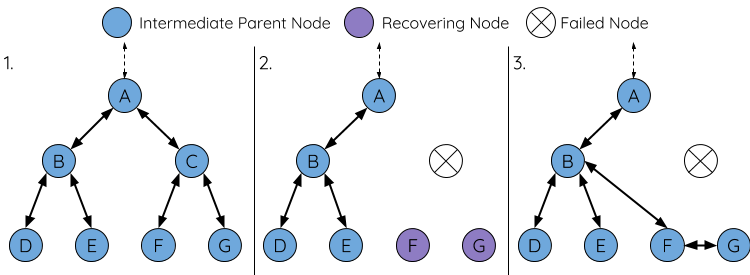
\includegraphics[scale=0.5]{images/mesh-parent-node-failure.png}
                        \caption{Défaillance d'un noeud intermédiaire\cite{esp-mesh_w}}
                    \end{figure}
            \end{itemize}
            \vspace{0.5cm}
            \textbf{Changement de racine}\newline
                Un changement de racine n'est possible que dans deux situations:
                \begin{enumerate}
                    \item La racine tombe. (voir point précédent)
                    \item La racine le demande via un appel à \textbf{esp\_mesh\_waive\_root()}.
                        Dans ce cas, un processus d'élection de racine sera initialisé. La nouvelle racine élue
                        enverra alors une \textit{switch request} à la racine actuelle qui répondra par un acquittement.
                        Ensuite la nouvelle racine se déconnectera de son parent et se connectera au routeur.
                        L'ancienne racine se déconnectera du routeur et deviendra un noeud idle pour enfin se connecter à un nouveau parent.
                \end{enumerate}
        \textbf{Paquets ESP-MESH}\\
            Les paquets \espmesh\ sont contenus dans une trame \wifi. Une transmission multi-sauts utilisera un paquet \espmesh\ transporté 
            entre chaque noeud par une trame \wifi\ différente.
            La figure \ref{fig_meshPacket} montre la structure d'un paquet \espmesh:\\

            \begin{figure}[h]
                \centering
                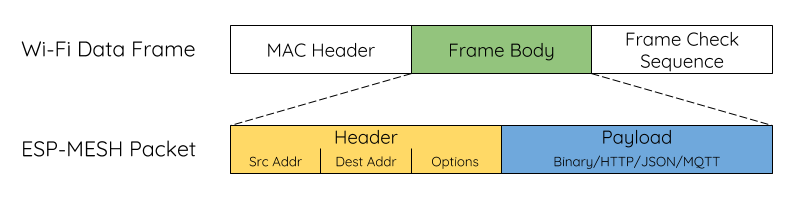
\includegraphics[scale=0.5]{images/mesh-packet.png}
                \caption{Paquet \espmesh\ \cite{esp-mesh_w}}
                \label{fig_meshPacket}
            \end{figure}
            Le header d'un paquet \espmesh\ contient les adresses source et destination ainsi que diverses options.
            Le payload d'un paquet \espmesh\ contient les données de l'application.

            Dans le cas où l'adresse de destination est une adrese \textsc{ip}, le paquet sera envoyé à la racine du réseau
            \espmesh\ qui transmet le payload du paquet (par exemple en initiant une connexion tcp avec un socket).
        \vspace{0.5cm}\\
        \textbf{Contrôle de flux}\\
            Pour éviter que les parents soient submergés de flux venant de leurs enfants, chaque parent va
            assigner une fenêtre de réception à chaque enfant. Chaque noeud enfant doit demander une fenêtre
            de réception avant chaque transmission. La taille de la fenêtre peut être ajustée dynamiquement.
            Une transmission d'un enfant vers un parent se déroule en plusieurs étapes:
            \begin{enumerate}
                \item Le noeud enfant envoit à son parent une requête de fenêtre. Cette requête contient le numéro de séquence du paquet en attente d'envoi.
                \item Le parent reçoit la requête et compare le numéro de séquence avec celui du précédent paquet envoyé par l'enfant.
                    La comparaison est utilisée pour calculer la taille de la fenêtre qui est transmise à l'enfant.\footnote{Ce calcul n'est pas précisé par Espressif}
                \item L'enfant transmet le paquet conformément à la taille de fenêtre spécifiée par le parent. Une fois la fenêtre de réception utilisée, l'enfant doit renvoyer une demande de fenêtre.
            \end{enumerate}
        \vspace{0.5cm}
        \textbf{Performances}\\
            Espressif fournit les performances d'\espmesh\ pour un réseau de maximum 100 noeuds, 6 couches et
            un nombre d'enfants par noeud de 6 (voir table \ref{performances_espMesh}).
            \begin{table}[H]
                \begin{tabular}{|l|l|}
                    \hline
                    Temps de construction du réseau & $<$ 60 secondes\\ \hline
                    Latence par saut & 10 à 30 millisecondes\\ \hline
                    Temps de réparation du réseau & \makecell{Si la racine tombe: $<$ 10 secondes \\ Si un noeud enfant tombe: $<$ 5 secondes}\\ \hline
                \end{tabular}
                \caption{Performances d'\espmesh\ \cite{esp-mesh_w}}
                \label{performances_espMesh}
            \end{table}
            \hspace{-0.75cm}
            \textbf{Discussion}\\
            A première vue, une topologie en arbre n'est pas robuste car si la racine tombe,
            tout le reste du réseau est déconnecté. Cependant le processus d'élection
            d'une nouvelle racine semble efficace selon les résulats fournis par Espressif.
            Un point négatif du protocole est que pour un noeud donné, sa table de routage contient tous les
            noeuds de son sous-arbre.
            On imagine donc difficilement utiliser ce protocole pour un nombre élevé de noeuds.

\chapter{AODV}
    Ad-hoc On-demand Distance Vector (\aodv) est un protocole réactif à vecteur de distance.
    Les 3 types de messages définis dans \aodv\ sont les Route requests (\textit{\rreq s}),
    les Route Remplies (\textit{\rrep s}) et les Route Errors (\textit{\rerr s}).
    Comme illustré sur la figure suivante, le premier sera envoyé en flooding par un noeud
    désirant obtenir une nouvelle route pour
    une desination donnée. Le second sert de réponse au premier. Il est envoyé à l'émetteur du
    \rreq. Et le dernier sert notamment lorsqu'un lien d'une route active est brisé. 
    Nous détaillons plus bas ces mécanismes.
    \vspace{1cm}
    \begin{figure}[H]
        \centering
        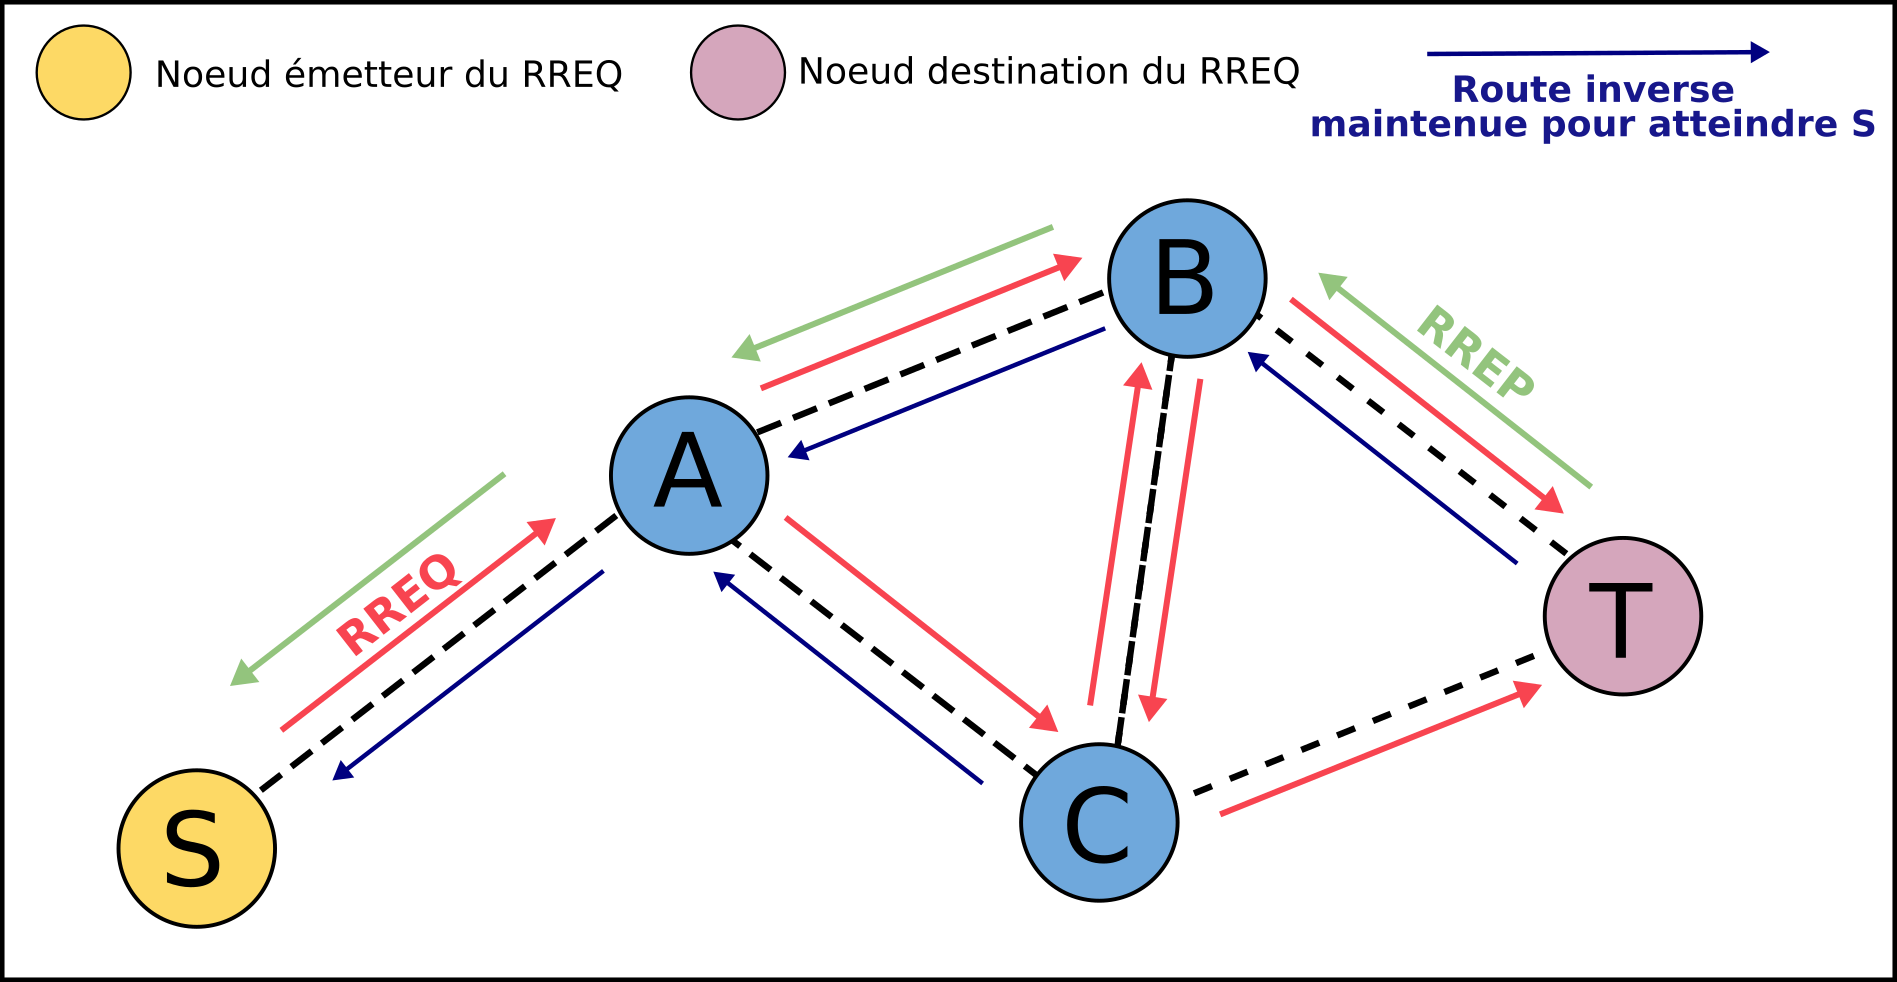
\includegraphics[scale=0.35]{images/aodv.png}
        \caption{Illusration du fonctionnement d'AODV}
        \label{aodv}
    \end{figure}
    
    
    \vspace{0.5cm}
    %\textbf{Format des paquets}\\
    \section{Format des paquets}
        \textbf{RREQ}\\
            \begin{figure}[H]
                \centering
                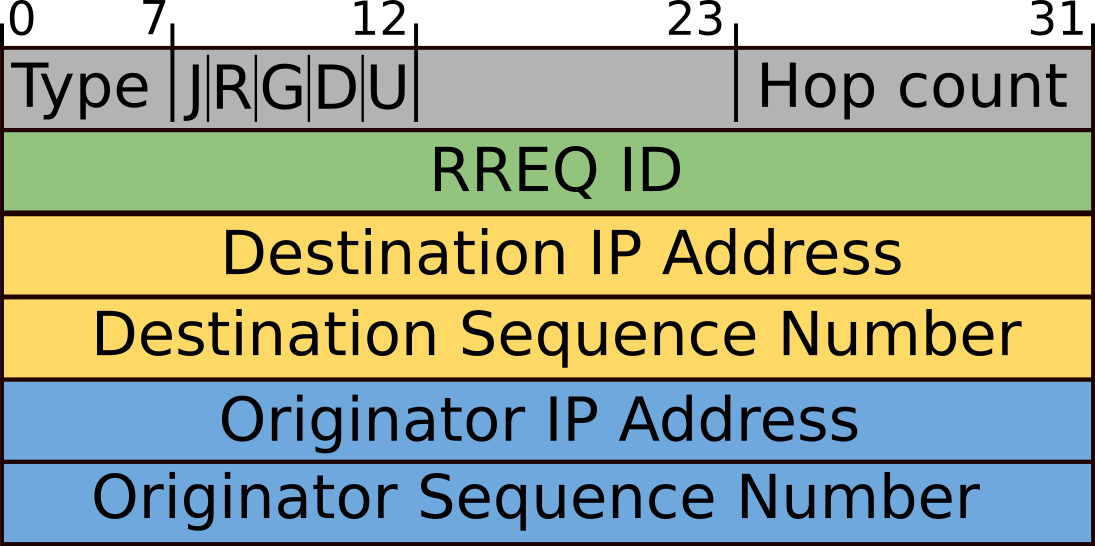
\includegraphics[scale=0.5]{images/rreq.png}
                \caption{Format d'un paquet \rreq\ \cite{rfc_aodv}}
                \label{rreqPaquet}
            \end{figure}
            Le format d'un \rreq\ est illustré sur la figure précédente. Il contient les champs
            repris dans la table suivante:\\
            \begin{table}[H]
                \begin{tabular}{ll}
                    type & \makecell[l]{$=1$}\\\hline
                    J R G & \makecell[l]{flags}\\\hline
                    D  & \makecell[l]{flag indiquant que seul la destination peut\\ répondre au \rreq}\\\hline
                    U & \makecell[l]{flag indiquant que le numéro de séquence de la\\ destination est inconnu}\\\hline
                    Hop count & \makecell[l]{nombre de sauts depuis le noeud source}\\\hline
                    \rreq\ \textsc{id} & \makecell[l]{numéro de séquence identifiant le \rreq}\\\hline
                    Destination IP Address & \makecell[l]{adresse \textsc{ip} du noeud pour lequel la route\\ est demandée}\\\hline
                    Destination Sequence Number & \makecell[l]{le dernier numéro de séquence connu pour une \\route vers la destination}\\\hline
                    Originator IP Address & \makecell[l]{adresse ip de l'émetteur du \rreq}\\\hline
                    Originator Sequence Number & \makecell[l]{numéro de séquence à utiliser pour une route\\ pointant vers l'émetteur du \rreq}\\
                \end{tabular}
                \caption{Champs d'un \rreq\ \cite{rfc_aodv}}
                \label{rreq_fields}
            \end{table}
            
        \textbf{RREP}\\
            \begin{figure}[H]
                \centering
                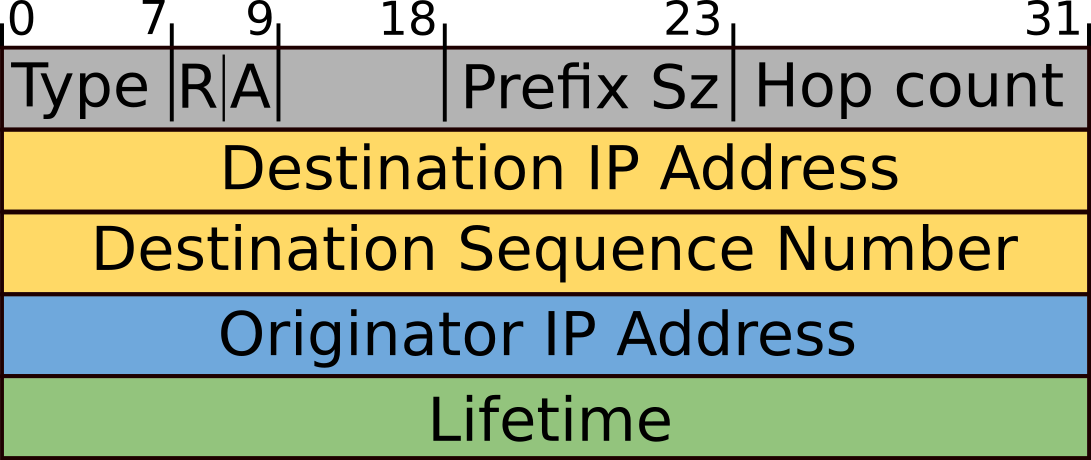
\includegraphics[scale=0.5]{images/rrep.png}
                \caption{Format d'un \rrep\ \cite{rfc_aodv}}
                \label{rreqPaquet}
            \end{figure}
            Le format d'un \rrep\ est illustré sur la figure précédente. Il contient les champs
            repris dans la table suivante:\\
            \begin{table}[H]
                \begin{tabular}{ll}
                    type & \makecell[l]{$=2$}\\ \hline
                    R & \makecell[l]{flag utilisé pour le multicast}\\ \hline
                    Prefix size & \makecell[l]{utilisé pour les aggrégations de routes}\\ \hline
                    Hop Count & \makecell[l]{nombre de sauts de l'\textit{originator} à la destination}\\ \hline
                    Destination IP address & \makecell[l]{adresse IP de du noeud pour qui l'adresse \\est demandée}\\ \hline
                    Destination Sequence Number & \makecell[l]{numéro de séquence de destination \\associé à la route}\\ \hline
                    Originator IP address & \makecell[l]{adresse IP du noeud émetteur du \rreq}\\ \hline
                    Lifetime & \makecell[l]{temps (en ms) pendant lequel le noeud qui reçoit \\le \rrep\ va considérer la route valide}\\
                \end{tabular}
                \caption{Champs d'un \rrep\ \cite{rfc_aodv}}
                \label{rrep_fields}
            \end{table}

    %\textbf{Découverte d'un chemin}\\
    \section{Découverte d'un chemin}
        La découverte d'un chemin est intiée par un noeud voulant envoyer des paquets à une destination pour laquelle il n'a aucune route valide.
        Chaque noeud possède deux compteurs: \textit{sequence\_number} et \textit{rreq\_id}.
        
        
        \vspace{0.5cm}
        \textbf{Génération du RREQ}\\
            Le noeud source incrémente ses compteurs \textit{sequence\_number} et \textit{rreq\_id} de 1.
            Il envoie ensuite un \rreq\ en broadcast à ses voisins.
        
        
        \vspace{0.5cm}
        \textbf{Propagation du RREQ}\\
            \begin{itemize}
                \item[$\bullet$] Noeud intermédiaire\\
                    A la réception d'un \rreq, un noeud intermédiaire va pouvoir rajouter ou mettre à jour
                    les routes vers son prédécesseur et vers le noeud source du \rreq.\\
                    Ensuite deux situations sont possibles:
                    \begin{enumerate}
                        \item Le noeud courant possède une route active vers la destination et le numéro de séquence de la route est plus grand 
                            ou égal au numéro de séquence de la destination dans le \rreq.
                            Dans ce cas, il peut envoyer par unicast un \rrep\ à la source du \rreq.
                        \item Sinon\\
                            Le noeud va incrémenter le nombre de sauts du \rreq\ et le propager à ses voisins.
                    \end{enumerate}

                \item[$\bullet$] Noeud destination\\
                    A la réception d'un \rreq\  lui étant destiné, un noeud va, comme un noeud intermédiaire, 
                    rajouter ou mettre à jour les routes vers son prédécesseur et vers le noeud source du \rreq.
                    Si le \textit{Destination Sequence Number} du \rreq\ est égal à son \textit{sequence\_number},
                    il va incrémenter ce dernier et envoyer un \rrep\ en unicast vers la source du \rreq.     
            \end{itemize}

        \vspace{0.5cm}
        \textbf{Propagation du RREP}\\
            A la réception d'un \rrep\ , un noeud va pouvoir rajouter ou mettre à jour
            les routes vers le noeud source du \rrep\  et vers son successeur.\\
            Il va ensuite incrémenter le nombre de sauts du \rrep\  et le propager en unicast vers la destination de ce \rrep\ .
            Cette propagation en unicast vers la source du \rreq\ est possible par l'apprentissage de la route inverse
            (destination du \rreq\ vers l'émetteur du \rreq) réalisée lors du flooding du \rreq.

    %\underline{\textbf{Table de routage}}\\
    \section{Table de routage}
        Chaque entrée d'une table de routage contient les informations suivantes:
        
        \begin{table}[H]
            \centering
            \begin{tabular}{|l|l|}
                \hline
                \textit{dest}       & Adresse IP de destination\\
                \textit{dest\_SN}   & Numéro de séquence de destination\\
                \textit{flag}       & Indicateur de numéro de séquence de destination valide\\
                \textit{out}        & Interface réseau\\
                \textit{hops}       & \makecell[l]{Comptage de sauts (nombre de sauts nécessaires\\ pour atteindre la destination)}\\
                \textit{next-hop}   & Prochain saut\\
                \textit{precursors} & Liste des précurseurs\\
                \textit{lifetime}   & temps d'expiration ou de suppression de l'itinéraire\\
                \hline
            \end{tabular}
            \caption{entrée d'une table de routage \aodv \cite{rfc_aodv}}
            \label{routingTable_aodv}
        \end{table}

        \textbf{Mise à jour de la table de routage}\\
            Soit N une nouvelle route et O la route existante.\\
            O est mise à jour si:\\
            \begin{center}
                \begin{tabular}{|l|}
                    \hline
                    $O.SN \leq N.SN$ \\
                    \textbf{ou} ($O.SN = N.SN$ \textbf{et} $O.hop\_count > N.hop\_count$)\\
                    \hline
                \end{tabular}
            \end{center}
        
        \textbf{Gestion du \textit{lifetime}}\\
            Le temps de vie d'une route dans la table de routage est initialisé à \textit{active\_route\_timeout} (3 millisecondes).\\
            Quand ce timer expire, la route passe de active à inactive. Une route inactive ne pourra plus être utilisée pour transférer des données
            mais pourra fournir des informations pour de futurs \rreq\  et la réparation de routes.\\
            Quand une route est utilisée, son temps de vie  est actualisé à: $current time + active\_route\_timeout$

    %\vspace{0.5cm}
    %\textbf{Evitement de boucles}\\
    \section{Evitement de boucles}
        A priori les numéros de séquences suffisent pour éviter les boucles. Cependant, d'après \cite{loop_aodv}, il y a des
        ambiguités dans le RFC \cite{rfc_aodv}. Dû à ces ambiguités, l'implémentation pourrait introduire des boucles.
        %Certaines parties du RFC concerant la gestion des numéros de séquences pourraient introduiredes boucles. 
        Nous approfondirons la lecture de cet article si nous choisissons ce protocole afin d'éviter les boucles dans notre implémentation.

        %\vspace{0.5cm}
    %\textbf{Défaillance d'un lien}\\
    \section{Défaillance d'un lien}
        Un noeud faisant partie d'une route active broadcast des messages \textit{hello} (\rrep)
        régulièrement.\\
        Si un noeud ne reçoit pas de message durant un certain temps pour un voisin, il va considérer
        que le lien avec ce voisin est perdu.\\
        Dans ce cas, il va en informé ses voisins impactés par un \textsc{rerr}.
    
    \section{Discussion}
        Ce protocole semble plus robuste que \espmesh. Car en comparaison avec ce dernier, si un noeud tombe,
        les noeuds peuvent trouver une autre route pour envoyer des pauqtes d'un point à un autre.
        A priori cette robustesse dépend également de certains paramètre comme le temps de vie ou la fréquence
        d'émission des messages \textit{hello}.
        

%\chapter{Implémentation}
%
%%%%%%%%%%%%%%%%%%%%%%%%%%%%%%%%%%%%%%%%%%%%%%%%%%%%%%%%%%%%%%%%%%%%%%%%%%%%%%%%
%\section{Limitations}
%        Le driver Wi-Fi d'\textit{IDF} ne nous permet pas d'avoir une connexion
%        avec plusieurs noeuds simultanément. \espnow\ pourraît être une solution
%        pour palier à ce problème.\\
%    
%    
%        \textbf{ESP NOW}\\
%            \espnow\ est un protocole de communication Wi-Fi sans connexion défini
%            par Espressif.\\ Nous n'avons trouvé aucune documentation décrivant le
%            fonctionnement de ce protocole.\\
%            Avec la documentation disponible, nous savons qu'un noeud a une liste
%            de \textit{peers} (ses voisins) avec qui il peut échanger des données.
%            Le nombre de voisins est limité à 20. Cette limite ne posera pas 
%            problème pour ce projet.
%        
%%%%%%%%%%%%%%%%%%%%%%%%%%%%%%%%%%%%%%%%%%%%%%%%%%%%%%%%%%%%%%%%%%%%%%%%%%%%%%%%
%\section{Prochaines étapes}
%        \begin{enumerate}
%            \item Nous allons créer un réseau \espmesh. Ceci nous permettra de nous
%            familiariser avec l'environnement \textit{IDF}.
%            \item Nous évaluerons les performances et fonctionnalités de ce protocole.
%            \item Nous implémenterons un protocole de routage mesh choisis plus haut.
%            \item L'objectif est de l'implémenter au niveau de la couche liaison de données.
%                Si nous rencontrons trop de difficulté ou que nous jugeons que ce 
%                choix n'est pas judicieux, nous implémenterons ce protocole au niveau 
%                de la couche réseau.
%            \item Nous étudierons les différentes possibilités d'économies d'énergie
%            \item Nous évaluerons les performances et fonctionnalités du prorotype créé. 
%            
%        \end{enumerate}

\chapter{Mise en oeuvre}
    \todo{INTRO}\\
    Nous avons utilisé la version 3.3.1 d'IDF car c'est une version stable suportée jusqu'en février 2022.
    \section{ESP-MESH}
    \begin{enumerate}
        \item \textbf{\underline{Construction du réseau}}\\
            Notre première étape a été d'établir un réseau \espmesh\ composé de deux noeuds (une racine et son enfant).
            Voici un extrait du code permettant de construire ce réseau:\newpage
            \begin{minted}[xleftmargin=\parindent,linenos]{c}
void app_main(void){
    /* stop DHCP server for softAP and station interfaces */
    ESP_ERROR_CHECK(tcpip_adapter_dhcps_stop(TCPIP_ADAPTER_IF_AP));
    ESP_ERROR_CHECK(tcpip_adapter_dhcpc_stop(TCPIP_ADAPTER_IF_STA));

    /* wifi initialisation */ 
    wifi_init_config_t config = WIFI_INIT_CONFIG_DEFAULT();
    ESP_ERROR_CHECK(esp_wifi_init(&config));
    ESP_ERROR_CHECK(esp_wifi_start());
    /*  mesh initialisation*/
    ESP_ERROR_CHECK(esp_mesh_init());
    mesh_cfg_t cfg = MESH_INIT_CONFIG_DEFAULT();
    /* event handler */
    cfg.event_cb = &mesh_event_handler;

            /* ... */
    
    /* set mesh configuration */
    ESP_ERROR_CHECK(esp_mesh_set_config(&cfg));
    /* mesh start */
    ESP_ERROR_CHECK(esp_mesh_start());
}
            \end{minted}
            On remarque que nous désactivons le serveur DHCP. En effet, la racine étant la passerelle entre 
            le réseau \espmesh\ et l'extérieur, elle est la seule à avoir besoin d'une adresse IP.
            Le serveur DHCP sera activé sur la racine une fois celle-ci élue.
            Ensuite le \wifi\ est initialisé ainsi que le réseau \espmesh, pour enfin démarrer ce dernier.\\
            Analysons la construction du réseau avec 2 noeuds:\\
            \begin{minted}[xleftmargin=\parindent,linenos]{console}
I (1479) mesh: <MESH_NWK_LOOK_FOR_NETWORK>need_scan:0x1, 
    need_scan_router:0x0, look_for_nwk_count:1
I (1779) mesh: [FIND][ch:7]AP:0, otherID:0, MAP:0, idle:0, 
    candidate:0, root:0[00:00:00:00:00:00]
I (1779) mesh: [FIND:1]fail to find a network, channel:0, 
    cfg<channel:7, router:MyRouter, 00:00:00:00:00:00>

I (1789) mesh: <MESH_NWK_LOOK_FOR_NETWORK>need_scan:0x3, 
    need_scan_router:0x1, look_for_nwk_count:2
I (1919) mesh: [S1]MyRouter, 1a:b2:c3:d4:e5:f6, channel:7, rssi:-43
I (1919) mesh: find router:[ssid_len:13]MyRouter, rssi:-43, 
    1a:b2:c3:d4:e5:f6(encrypted), new channel:7, old channel:0
I (1929) mesh: [FIND][ch:7]AP:1, otherID:0, MAP:0, idle:0, candidate:0, 
    root:0[1a:b2:c3:d4:e5:f6]router found<scan router>
I (1939) mesh: [FIND:2]find a network, channel:7, cfg<channel:7, 
    router:MyRouter, 00:00:00:00:00:00>

I (1949) wifi: mode : sta (3c:71:bf:0d:83:08) + softAP (3c:71:bf:0d:83:09)
I (2269) mesh: [SCAN][ch:7]AP:2, other(ID:0, RD:0), MAP:1, idle:1,
    candidate:1,root:0, topMAP:0[c:1,i:1][1a:b2:c3:d4:e5:f6]router found<>
I (2269) mesh: 1022<pre>my_vote_num:0, voter_num/max_connection:4,
    2nd_layer_count:0
I (2279) mesh: 6104[SCAN]init rc[ttl:127/votes:1][3c:71:bf:0d:7e:1d,-120]
I (2279) mesh: 6104[SCAN]init rc[ttl:127/votes:1][3c:71:bf:0d:7e:1d,-120]
I (2289) mesh: 1250, vote myself, router rssi:-45 > voted rc_rssi:-120
I (2299) mesh: [SCAN:1/10]rc[128][3c:71:bf:0d:83:09,-45], 
    self[3c:71:bf:0d:83:08, -45,reason:0,votes:1,idle]
        [mine:1,voter:1(1.00)percent:0.90][128,1,3c:71:bf:0d:83:09]

                            ....
I (8049) mesh: [SCAN:10/10]rc[128][3c:71:bf:0d:83:09,-45], 
    self[3c:71:bf:0d:83:08,-39,reason:0,votes:2,idle][mine:2,voter:2(1.00)percent:0.90][128,2,3c:71:bf:0d:83:09]

I (8069) mesh: [DONE]connect to router:Sitecom0BD453, channel:7,
    rssi:-39, 64:d1:a3:0b:d4:53[layer:0, assoc:0], my_vote_num:2/voter_num:2, rc[3c:71:bf:0d:83:09/-45/1]
                            

            \end{minted}
            On remarque d'abord que le noeud cherche un réseau \espmesh. Comme il n'en trouve pas,
            il va chercher un point d'accès. Il trouve le point d'accès \textit{"MyRouter"} qui est sur 
            le canal 7 et avec lequelil a un \rssi\ de -43. Ensuite il écoute les beacons
            des autres noeuds. On remarque bien qu'il détecte un autre noeud idle.
            Ensuite le vote commence à la ligne 19. À chaque itération du vote, le noeud
            écoute les beacons des autres noeuds. Ici il en détecte un autre noeud idle qui a un \rssi
            avec le routeur de -120. Comme $-45 > -120$, il va voter pour lui-même. Ce qui veut dire émettre
            un beacon avec ses informations. Si son \rssi\ était moins fort que celui de l'autre noeud, 
            il aurait émis un beacon avec les informations de l'autre noeud. Ce que nous avons décrit ici
            correspond à une itération du vote. Dans notre cas il y aura 10 itérations. Ce nombre est un paramètre
            tu réseau \espmesh. A la fin des 10 itérations, le noeud compare son ratio au seuil (ici de 0.90).
            Comme ce ratio ( ici 1) est plus grand que le seuil, le noeud devient la racine du réseau \espmesh\ et 
            se connecte au routeur.
            Ses observations correspondent bien à la description du protocole faite plus haut.

            Nous avons également observer la construction du réseau avec Wireshark. On remarque bien cet échange
            de beacons. Voici un exemple du contenu d'un beacon:\\
            \begin{alltt}
0000 00 00 1a 00 2f 48 00 00 27 b3 bb 07 00 00 00 00
0010 10 02 8a 09 a0 00 de 00 00 00 \textcolor{red}{80 00 00 00 ff ff
0020 ff ff ff ff 3c 71 bf 0d 83 09 3c 71 bf 0d 83 09
0030 10 00} db 9c 01 00 00 00 00 00 64 00 21 04 00 00
0040 01 08 8b 96 82 84 0c 18 30 60 03 01 07 05 05 01
0050 02 00 00 00 07 06 43 4e 00 01 0d 14 2a 01 00 32
0060 04 6c 12 24 48 2d 1a 6e 11 00 ff 00 00 00 00 00
0070 00 00 00 00 00 00 01 00 00 00 00 00 00 00 00 00
0080 00 3d 16 07 05 00 00 00 00 00 00 00 00 00 00 00
0090 00 00 00 00 00 00 00 00 00 dd 18 00 50 f2 02 01
00a0 01 04 00 03 a4 00 00 27 a4 00 00 42 43 5e 00 62
00b0 32 2f 00 \textcolor{blue}{dd 45 18 fe 34 01 02 00 77 77 77 77 77
00c0 77 19 00 04 00 00 00 00 00 00 00 00 00 00 00 88
00d0 88 00 00 00 00 00 00 00 88 00 00 00 00 00 00 88
00e0 00 00 00 00 00 00 00 00 00 00 00 00 00 00 00 0a
00f0 00 00 00 0f 00 00 5f 8a d2 40 dd 16 18 fe 34 06
0100 02 00 0b 45 53 50 4d 5f 30 44 38 33 30 38 cd 20
0110 f9 23 dd 15 18 fe 34 0c 02 00 00 00 00 00 00 6d
0120 ef a8 4d 99 5c 80 b0 d2 d3} a1 d2 b2 10
            \end{alltt}

            En rouge, nous avons l'entête 802.11 et en bleu les paramètres supplémentaires
            d'Espressif pour le réseau \espmesh.
            Dans l'entête 802.11, on remarque l'adresse de destination qui est l'adresse Broadcast
            ainsi que l'adresse source qui est celle du noeud qui a émis ce beacon.
            Dans les paramètres supplémentaires, nous avons seulement distinguer l'id du réseau
            \espmesh\ qui est 77 77 77 77 77 77. 
            

        

        \item \textbf{\underline{Communications internes}}\\
            La deuxième étape a été de faire communiquer ses deux noeuds. Nous avons donc envoyer des
            messages \espmesh\ de la feuille vers la racine.
            Pour repérer plus facilement les paquets \espmesh\ dans Wireshark, nous avons envoyé
            20 fois $238$ ce qui vaut $EE$ en hexadécimal.
            Une fois l'évènement MESH\_EVENT\_PARENT\_CONNECTED détecté, les communications sont initialisées
            en fonction que le noeud soit la racine ou non. Nous obtenons cette infrmation via \textbf{{esp\_mesh\_is\_root()}}
            \begin{itemize}
                \item Pour la racine: Le serveur DHCP et une tâche FreeRTOS (créer via \textbf{{xTaskCreate()}})
                sont démarrés. Cette tâche écoute en permanance les paquets \espmesh\ qui sont destinés au noeud via la méthode
                \textbf{{esp\_mesh\_recv()}}.
                \item Pour les autres types de noeuds du réseau, une tâche FreeRTOS est démarrée. Cette tâche envoie continuellement
                des paquets \espmesh\ contenant 20 fois EE comme données à la racine. Cet envoi ce fait via la méthode
                \textbf{{esp\_mesh\_send()}}.
            \end{itemize}
            Voici un extrait du code réalisant ce que nous venons d'expliquer:
            \begin{minted}[xleftmargin=\parindent,linenos]{c}
void esp_mesh_rx(void *arg){
    esp_err_t err;
    uint8_t rx_buf[RX_BUF_SIZE]={0,}; //receive buffer
    mesh_addr_t from; //src addr
    int flag = 0;
    
    /* mesh data */
    mesh_data_t data;
    data.data = rx_buf;
    data.size = sizeof(rx_buf);

    while(){
        /* recv
         *  - from addr
         *  - data
         *  - timeout in ms (0:no wait, portMAX_DELAY:wait forever)
         *  - flag
         *  - options
         *  - number of options
         **/
        err = esp_mesh_recv(&from, &data, 5000, &flag, NULL, 0);
        if(err == ESP_OK){
            printArray(rx_buf, RX_BUF_SIZE);
        }
    }
    /* delete the task */
    vTaskDelete(NULL); 
}
void esp_mesh_tx(void *arg){
    esp_err_t err;

    static uint8_t tx_buf[TX_BUF_SIZE]= {238, 238, 238, 238, 238, 238, 238, 238, 238, 238, 238, 238, 238, 238, 238, 238, 238, 238, 238, 238};
    
    /* mesh data */
    mesh_data_t mesh_data;
    mesh_data.data = tx_buf;
    mesh_data.size = sizeof(tx_buf);
    mesh_data.proto = MESH_PROTO_BIN;

    while(){
        /* send:
         *  - dest addr
         *  - data: NULL for the root
         *  - flag
         *  - options
         *  - number of options
         **/
        err = esp_mesh_send(NULL, &mesh_data, 0, NULL, 0);
    }
    /* delete the task */
    vTaskDelete(NULL);
}
void esp_mesh_comm_p2p_start(){
    static bool p2p_started = false;
    if(!p2p_started){
        if(esp_mesh_is_root()){// root node
            xTaskCreate(esp_mesh_rx, "MPRX", 3072, NULL, 5, NULL);       
        }else{// intermediate or leaf node
            xTaskCreate(esp_mesh_tx, "MPTX", 3072, NULL, 5, NULL);
        }
    }
}

void mesh_event_handler(mesh_event_t event){
    if (event.id == MESH_EVENT_PARENT_CONNECTED){
        if (esp_mesh_is_root()) {
            /* start DHCP server for the root node */
            tcpip_adapter_dhcpc_start(TCPIP_ADAPTER_IF_STA);
        }
        esp_mesh_comm_p2p_start();
    }
}
            \end{minted}
            Analysons les communications:\\
            Grâce aux données que nous avons choisies d'envoyer, nous avons repérer facilement
            les paquets avec lequels ces données sont envoyées. Pour cet exemple de paquet,
            nous avons utilisé 3 noeuds: La racine, un noeud intermédiaire et une feuille.
            La feuille envoie un paquet à la racine.
            \begin{alltt}
0000   00 00 1a 00 2f 48 00 00 b0 23 e1 04 00 00 00 00
0010   10 02 8a 09 a0 00 e2 00 00 00 \textcolor{red}{88 01 3a 01 3c 71
0020   bf 0d 83 09 3c 71 bf 0d 7e 18 3c 71 bf 0d 83 09
0030   50 00 00 00} \textcolor{ForestGreen}{aa aa 03 18 fe 34 ee ee} \textcolor{blue}{21 07 30 00
0040   31 04 40 01 00 00 00 00 00 00 3c 71 bf 0d 7e 18
0050   02 00 00 00 02 00 00 00 ee ee ee ee ee ee ee ee
0060   ee ee ee ee ee ee ee ee ee ee ee ee} f8 5e 65 af
                
            \end{alltt}
            En rouge nous avons l'entête 802.11 où nous pouvons distinguer les adresses
            \mac\ du noeud source et du noeud de destination.
            En vert, Nous trouvons la couche \todo{bof} \textsc{llc} (logical link control)
            qui agit comme interface entre la couche \mac\ et la couche réseau.
            Enfin en bleu, le paquet \espmesh\ contenant:
            \begin{itemize}
                \item 8 octets que nous supposons être utilisés pour des options
                \item 6 octets utilisés pour l'adresse de destination (cette adresse est celle
                utilisée pour la racine du réseauenumerate).
                \item 6 octets utilisés pour l'adresse source
                \item 8 octets que nous supposons être utilisés pour des options
                \item 20 octets utilisés pour notre payload
            \end{itemize}
            La taille maximale du payload (\textsc{mps}) est de 1472 octets. Le total nous donne donc 1500
            octets ce qui correspond bien au \textsc{mtu} défini pour \espmesh.
            \footnote{Les constantes MTU et MPS sont définies dans le fichier \textbf{esp\_mesh.h}}
 
        \item \textbf{\underline{Communications externes}}\\
            \todo{\~\ extérieur}\\
            Comme nous l'avons déja dit plus haut, la racine joue le rôle de passerelle entre le réseau \espmesh\ 
            et l'extérieur. Lorsqu'elle reçoit des données pour l'extérieur, elle va initier une communication avec l'adresse
            de destination via des socket. L'implémentation de la couche IP avec IDF est lwIP (lightweight IP). lwIP est
            une implémentation légère de la couche IP adaptée aux systèmes embarqués. Pour nous familiariser à l'utilisation
            de socket avec lwIP, nous avons d'abord réalisé une communication TCP entre un \esp\ et un Raspberry pi utilisé
            comme serveur. Voici un extrait de code: 
            \begin{minted}[xleftmargin=\parindent,linenos]{c}
void mySend(){

    /* set dest addr */
    struct sockaddr_in destAddr;
    destAddr.sin_addr.s_addr = inet_addr(DEST_ADDR);
    destAddr.sin_port = htons(DEST_PORT);
    destAddr.sin_family = AF_INET;

    /* set src addr */
    struct sockaddr_in srcAddr;
    srcAddr.sin_port = htons(SRC_PORT);
    srcAddr.sin_family = AF_INET;
    //get station info
    tcpip_adapter_ip_info_t ipInfo;
    esp_err_t r = tcpip_adapter_get_ip_info(TCPIP_ADAPTER_IF_STA, &ipInfo);
    //set srcAddr IP to station IP
    memcpy((u32_t *) &srcAddr.sin_addr, &ipInfo.ip.addr, 
        sizeof(ipInfo.ip.addr));

    /* create TCP socket */
    int sock = socket(AF_INET, SOCK_STREAM, IPPROTO_IP);

    /* bind socket to srcAddr */
    bind(sock, (struct sockaddr *)&srcAddr, sizeof(srcAddr))

    /* connect socket to destAddr */
    connect(sock, (struct sockaddr *) &destAddr, sizeof(destAddr))

    /* send data */
    send(sock, payload, sizeof(payload), 0)
}
            \end{minted}

            Tout d'abord, nous créons les adresses sources et destinations. Comme la source sera notre \esp,
            nous récupérons son adresse IP via \textbf{tcpip\_adapter\_get\_ip\_info()} auquel nous demandons
            les informations de l'interface \textit{station}. Ensuite, nous pouvons créer un socket, le lier à l'adresse
            source et enfin le connecter à la destination pour pouvoir envoyer des données.

            
            Ensuite nous avons rajouter la possibilité pour les noeuds du réseau \espmesh\ d'envoyer des paquets vers l'extérieur.
            Lorsqu'un message destiné à une adresse IP externe est reçu par la racine, il est récupéré via la fonction
            \textbf{esp\_mesh\_recv\_toDS()}. Nous devons ensuite créer un socket TCP avec comme adresse source, celle de la racine
            et comme adresse destination, celle spécifié dans le paquet \espmesh\ reçu par la racine.
            Voici l'extrait de code qui nous intéresse:
            \begin{minted}[xleftmargin=\parindent,linenos]{c}
mesh_addr_t mesh_to_addr;
struct sockaddr_in ip_to_addr;

err = esp_mesh_recv_toDS(&mesh_from_addr, &mesh_to_addr, &mesh_data, 
    timeout, &flag, NULL, 0);

memcpy((u32_t *) &ip_to_addr.sin_addr, &mesh_to_addr.mip.ip4.addr,
    sizeof(mesh_to_addr.mip.ip4.addr));
/*create, bind and connect socket*/
sock_error = send(sock, mesh_data.data, mesh_data.size, 0);
                
            \end{minted}
            Une difficulté a été la ligne 7 car il a fallu connaître le type de l'adresse IP du paquet \espmesh\ 
            ainsi que celui de l'adresse de \textit{sockaddr\_in}.

            \todo{SOCKET SELECT}
        
        \item \textbf{\underline{Extension à Wireshark}}\\
        
    \end{enumerate}

    \section{ESP-NOW}
        Le driver Wi-Fi d'\textit{IDF} ne nous permet pas d'avoir une connexion avec plusieurs noeuds simultanément. 
        Nous supposons que c'est pour cette raison qu'\espmesh\ utilise une structure d'arbre et non de graphe.
        \espnow\ est une solution qui palie à ce problème.\\
        En effet un noeud peut avoir maximum 20 voisins. Ce qui est suffisant pour établir un réseau \mesh\ tel
        que nous l'envisagons. Par contre comparé à \espmesh, le \textsc{mtu} est plus petit. En effet il est
        de 250 octets.\footnote{le \textsc{mtu} et le nombre de voisins maximum sont définis dans le fichier
        \textbf{esp\_now.h}}

        Utilisons \espnow:\\
        Nous avons utilisés 3 noeuds. Un des noeuds envoie des données en broadcast aux autres.
        Voici un exrait du code permettant de réalisé ce que nous venons de décrire:
        \begin{minted}[xleftmargin=\parindent,linenos]{c}

#define ESPNOW_WIFI_MODE WIFI_MODE_STA // Wi-Fi mode: sta, ap or sta+ap
#define ESPNOW_WIFI_IF ESP_IF_WIFI_STA // Wi-Fi interface sta or ap

static const uint8_t broadcast_addr[ESP_NOW_ETH_ALEN] = 
    {0xFF, 0xFF, 0xFF, 0xFF, 0xFF, 0xFF};

void espnow_recv_cb(const uint8_t *mac_addr, const uint8_t *data,
    int data_len){
    ESP_LOGI(TAG, "receive %d bytes:", data_len);
    printArray(data, data_len);
}

void esp_now_tx(void *arg){
            /* ... */
    /* create peer broadcast */
    esp_now_peer_info_t peer;
    peer.channel = CHANNEL;
    peer.ifidx = ESPNOW_WIFI_IF;
    peer.encrypt = false;
    memcpy(peer.peer_addr, broadcast_addr, ESP_NOW_ETH_ALEN);
    ESP_ERROR_CHECK(esp_now_add_peer(&peer)); // add peer

    ESP_LOGI(TAG, "send to all nodes");
    while(is_running){
        esp_now_send(&broadcast_addr, &data, sizeof(data));
        vTaskDelay( 1000 / portTICK_PERIOD_MS ); // delay the task
    }
    vTaskDelete(NULL); 
}

void app_main(void){    
            /* ... */
    /* Wi-Fi initialization */
    wifi_init_config_t config = WIFI_INIT_CONFIG_DEFAULT();    
    ESP_ERROR_CHECK(esp_wifi_init(&config));
    ESP_ERROR_CHECK(esp_wifi_set_mode(ESPNOW_WIFI_MODE));
    ESP_ERROR_CHECK(esp_wifi_start());
    
    /* ESP-NOW initialization */
    ESP_ERROR_CHECK(esp_now_init());
    ESP_ERROR_CHECK(esp_now_register_recv_cb(espnow_recv_cb));
            /* ... */
}
        \end{minted}
Tout d'abord nous initialisons le driver \wifi. Nous définissions le mode du driver \wifi\ à
\textit{station}. Cette interface sera utilisée par \espnow. Il est également possible d'utiliser 
l'interface \textit{acces point}. 
Ensuite nous définissions la fonction qui sera appellée lorsqu'un paquet \espnow\ est reçu.
Nous créons ensuite, pour le noeud source, la tâche \textbf{esp\_now\_tx()} qui envoie les données en broadcast.
Pour cela, nous devons d'abord créer un "voisin" broadcast, pour ensuite envoyer les données vers ce voisin.
Pour envoyer des données vers un noeud précis, il faut créer un voisin avec l'adresse \mac\ du noeud.

Pour construire un réseau \mesh, il faudrait, par exemple que chaque nouveau noeud émette en broadcast, un paquet \espnow\ 
contenant au moins son adresse \mac. De cette façons, les noeuds voisins pourraient le rajouter à leurs
liste de voisins.


%\listoffigures


\appendix
\addcontentsline{toc}{chapter}{Annexes}
\chapter{Multicasting et Broadcasting avec \espmesh}
\label{annexeA}
\textbf{Multicasting}\\
    Le multicasting permet d'envoyer simultanément un paquet \espmesh\ à plusieurs noeuds du réseau. Le multicasting
    peut être réalisé en spécifiant
    \begin{itemize}
        \item Soit un ensemble d'adresses \mac\\
            Dans ce cas, l'adresse de destination doit être
            {\fontfamily{qcr}\selectfont \textls[-300]{\small 0 1 : 0 0 : 5 E : x x : x x : x x}}
            Cela signifie que le paquet est un paquet multicast et que la liste des adresses peut être obtenue dans les options du header.
        \item Soit un groupe préconfiguré de noeuds\\
            Dans ce cas, l'adresse de destination du paquet doit être l'ID\footnote{Dans un réseau \espmesh, chaque groupe a un ID unique
            ayant la même structure qu'une adresse mac (par exmple {\small 7 7 : 7 7 : 7 7 : 7 7 : 7 7 : 7 7})}
            du groupe et un flag \textsc{mesh\_data\_group} doit être ajouté. % todo ajouté où ?
            % todo comment les noeuds sont au courant qu'ils sont dans ce groupe
    \end{itemize}

\vspace{0.5cm}
\textbf{Broadcasting}\\
    Le broadcasting permet de transmettre un paquet \espmesh\ à tous les noeuds du réseau. Pour éviter de gaspiller de
    la bande passante, \espmesh\ utilise les règles suivantes:
    \begin{enumerate}
        \item Quand un noeud intermédiare reçoit un paquet broadcast de son parent, il va le transmettre à tous ses enfants
            et en stocker une copie
        \item Quand un noeud intermédiaire est la source d'un paquet broadcast, il va le transmettre à son parent et à ses enfants
        \item Quand un noeud intermédiaire reçoit un paquet d'un de ses enfants, il va le transmettre à ses autres enfants, son parent
            et en stocker une copie
        \item Quand une feuille est la source d'un paquet broadcast, elle va le transmettre à son parent
        \item Quand la racine est la source d'un paquet broadcast, elle va le transmettre à ses enfants
        \item Quand la racine reçoit un paquet broadcast de l'un de ses enfants, elle va le transmettre à ses autres enfants et en stocker une copie
        \item Quand un noeud reçoit un paquet broadcast avec son adresse \mac\ comme adresse source, il l'ignore
        \item Quand un noeud intermédiaire reçoit un paquet broadcast de son parent, s'il possède une copie de ce paquet (càd que ce paquet a été à l'origine transmis par l'un de ses enfants), il va l'ignorer
            pour éviter les cycles ( protocole d'inondation)
    \end{enumerate}
\newpage

\chapter{Extrait de code de notre "proxy"}
\label{annexeB}
\begin{minted}[xleftmargin=\parindent,linenos]{c}
    void esp_mesh_external_rx(void *arg){
       struct sockaddr_in src;
       socklen_t sockLen;
   
       mesh_addr_t mesh_dest_addr;
       mesh_data_t mesh_data;
       mesh_data.proto = MESH_PROTO_BIN;
   
       uint8_t *mac_addr;
       static fd_set readSet;//set of file descriptors
       struct timeval timeout = {.tv_usec = 500000/*in microseconds*/};
       while(is_running){
           FD_ZERO(&readSet);//clear the set
           /*add sockets from the matching table to the set*/
           for(int i=0; i<MATCHING_TABLE_SIZE; i++){
               /*...*/
               currentSock=matching_table[i]->sock;
               FD_SET(currentSock,&readSet);
               /*...*/
           }
           if(select(maxSock+1, &readSet, NULL, NULL, &timeout) < 0){
               ESP_LOGE(TAG, "select error");
               continue;
           }
           /*search for the record that corresponds to the socket that
            *received data
            */
           for(int i=0; i<MATCHING_TABLE_SIZE; i++){
               /*...*/
               sock = matching_table[i]->sock;
               mac_addr = matching_table[i]->addr;  
               if(FD_ISSET(sock, &readSet)){//we found the record
                   recv_value = recvfrom(sock, rx_buf, sizeof(rx_buf), 0,
                       &src, &sockLen);
                   /*...*/
                   mesh_data.size = sizeof(rx_buf);//set mesh data
                   mesh_data.data = rx_buf;
                   memcpy(mesh_dest_addr.addr, mac_addr, 6);//set mesh addr
                   /*send data*/
                   err=esp_mesh_send(&mesh_dest_addr,&mesh_data,
                       MESH_DATA_P2P,NULL,0);
                   /*...*/      
               
               \end{minted}

\chapter{Code de notre dissecteur}
\label{annexeC}
\begin{minted}[xleftmargin=\parindent,linenos]{lua}
esp_mesh = Proto("ESP-MESH", "ESP-MESH Protocol")

dest_addr = ProtoField.ether("espmesh.dest", "Destination address", base.HEX)
src_addr = ProtoField.ether("espmesh.src", "Source address", base.HEX)
data = ProtoField.bytes("espmesh.data", "Data", base.NONE)
flags = ProtoField.bytes("espmesh.flags", "Flags", base.NONE)


esp_mesh.fields = {data, dest_addr, src_addr, flags}

local espmesh_PID = 0xeeee 

local data_data = Field.new("data.data")
local llc_pid = Field.new("llc.pid")

function esp_mesh.dissector(tvbuf, pinfo, tree)
    local llc_pid_ex = llc_pid()

    if llc_pid_ex == nil or data_data() == nil or llc_pid_ex.value ~= espmesh_PID then
        return
    end
    pinfo.cols.protocol:set("esp-mesh")

    local data_tvb = data_data().range()
    local esp_mesh_tree = tree:add(esp_mesh, data_tvb(0, data_tvb:len()))

    esp_mesh_tree:add(dest_addr, data_tvb(8, 6))
    esp_mesh_tree:add(src_addr, data_tvb(14, 6))
    esp_mesh_tree:add(flags, data_tvb(20, 8))
    if data_tvb:len() > 28 then
        esp_mesh_tree:add(data, data_tvb(28))
    end
end

register_postdissector(esp_mesh)
\end{minted}

\bibliography{bibliography}{}
\bibliographystyle{plain}

\end{document}